\documentclass[journal]{IEEEtran}
\IEEEoverridecommandlockouts

\usepackage{cite}
\usepackage{amsmath,amssymb,amsfonts}
%\usepackage{algorithm}
\usepackage{algorithmic}
\usepackage{graphicx}
\usepackage{textcomp}
\usepackage{xcolor}
\usepackage{tabularx}
\usepackage{booktabs}
\usepackage[colorlinks,linkcolor=red,anchorcolor=red,citecolor=blue]{hyperref}
\usepackage[lined,boxed,ruled]{algorithm2e}

\usepackage{tikz}
\usetikzlibrary{shapes.geometric, arrows.meta, positioning, fit, backgrounds, calc}
\usetikzlibrary{arrows.meta, positioning, shapes.geometric, shadows, patterns}

\usetikzlibrary{shapes.geometric, fit, backgrounds, arrows.meta}

\usepackage{pgfplots}
\pgfplotsset{compat=1.18}

\graphicspath{{./figs/}}

\def\BibTeX{{\rm B\kern-.05em{\sc i\kern-.025em b}\kern-.08em
    T\kern-.1667em\lower.7ex\hbox{E}\kern-.125emX}}
\begin{document}

\title{PaperProof: Decentralized Paper Publishing and Verification on Sui and Walrus}

\author{\IEEEauthorblockN{PaperProof Labs}\\
\IEEEauthorblockA{
paperproof.labs@gmail.com
}
}
\IEEEaftertitletext{\vspace{-1\baselineskip}}
\maketitle

\begin{abstract}
PaperProof is a live decentralized paper publishing and verification system for academic PDF documents built on Sui and Walrus. It provides an end-to-end workflow in which an author first reserves a unique on-chain paper identifier, then stamps that identifier into the PDF locally in the browser, uploads the final artifact to Walrus, and finalizes publication on Sui with metadata, storage references, and a cryptographic file hash. In this model, the canonical published object is not the original local source file, but the final stamped PDF that is actually released, retrieved, and later verified.

The system combines a static public website, browser-side PDF processing, a Sui Move contract, Walrus programmable storage, and OpenZeppelin-assisted administrative handoff into a unified publication pipeline. PaperProof supports explicit publication states, append-only version management, public lookup by paper code, and independent verification of downloaded artifacts against the on-chain hash record. It also adopts a lightweight governance route in which a governance committee determines the operational administrator, while administrative succession is secured through OpenZeppelin \texttt{two\_step\_transfer}.

A working mainnet deployment demonstrates that decentralized infrastructure can support practical scholarly publication and artifact provenance without relying on a centralized backend as the ultimate source of publication truth. Rather than attempting to replace peer review or broader academic governance, PaperProof focuses on a narrower but foundational systems problem: how to create, publish, preserve, retrieve, and verify scholarly PDF artifacts in a trust-minimized and publicly deployable manner.
\end{abstract}

\begin{IEEEkeywords}
decentralized scholarly publishing, scholarly artifacts, paper verification, Sui, Walrus, OpenZeppelin, programmable storage
\end{IEEEkeywords}

\section{Introduction}

Academic papers are now created, shared, revised, and circulated primarily through digital platforms. Yet most publication and preprint workflows still rely on centralized infrastructures for identifier issuance, metadata management, file hosting, and version presentation. These systems are efficient and familiar, but they also make the platform itself the primary authority for publication state, artifact identity, and long-term accessibility. In practice, this means that when a reader downloads a paper from a conventional platform, trust in the artifact is largely trust in the platform.

For scholarly communication, that trust boundary matters. A publication workflow should ideally provide a stable identifier, a visible and auditable release state, a durable link between metadata and the released document, and a clear way to verify that the retrieved file is exactly the artifact associated with the publication event. In many existing systems, however, these properties are only partially realized. A paper may have a stable landing page but no independently verifiable binding to the final distributed PDF. Version history may be visible but not preserved as append-only, artifact-specific publication state. Long-term artifact accessibility may depend almost entirely on the continued operation of the hosting service. As a result, the publication record and the released PDF often remain verifiable only within the platform's own trust boundary.

\begin{figure*}[!ht]
    \centering
    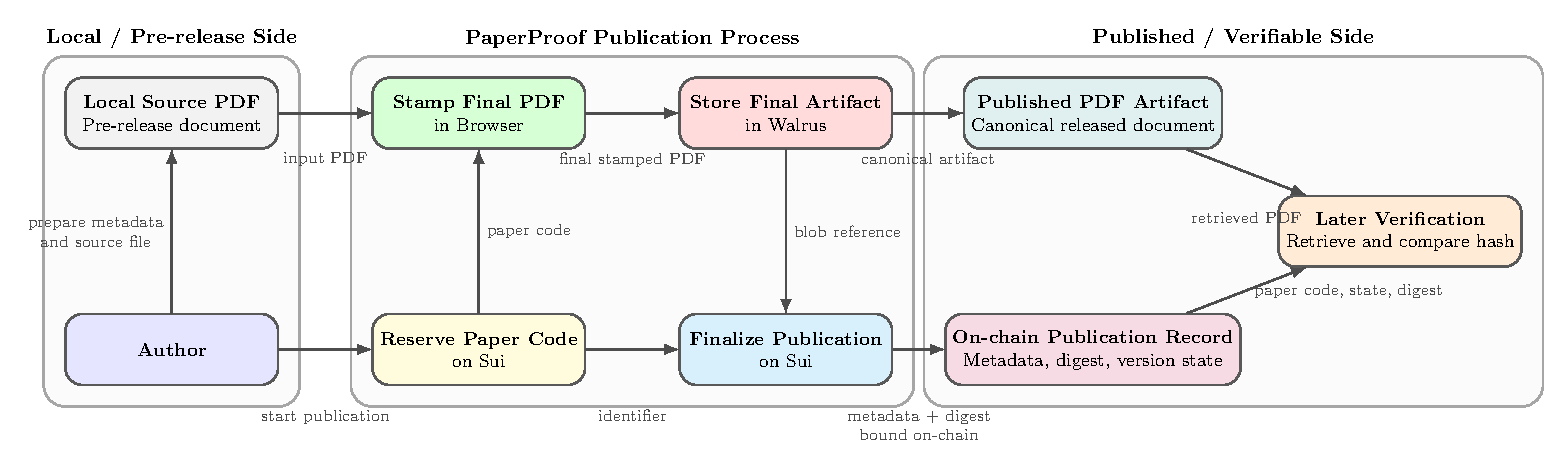
\includegraphics[width=0.92\textwidth]{introduction.pdf}
    \caption{Core publication concept of PaperProof. A local source PDF is transformed into a verifiable published artifact by reserving a paper code on Sui, stamping the final PDF in the browser, storing the canonical released artifact in Walrus, and binding publication metadata and file digest on-chain for later verification.}
    \label{fig:introduction_concept}
\end{figure*}


PaperProof is designed to change that boundary. This work presents \emph{PaperProof}, a live decentralized paper publishing and verification system for academic PDF documents built on Sui and Walrus. Rather than treating publication as a simple file upload followed by metadata display, PaperProof models publication as a trust-minimized artifact workflow. A unique paper code is first reserved on-chain. That code is then embedded into the PDF locally in the browser, producing the final released artifact. The stamped PDF is uploaded to Walrus, while its metadata, storage references, and cryptographic file hash are finalized on Sui. In this design, the canonical publication artifact is not the original local source file, but the final stamped PDF that is actually released, stored, retrieved, and later verified.

This publication model is based on three core ideas. First, publication is identifier-first: the paper code exists before the final artifact is formed. Second, publication truth is bound to the final released PDF rather than to a pre-release local file. Third, paper evolution is represented through append-only version records rather than overwrite-style updates. Together, these choices give PaperProof a publication model in which artifact identity, lifecycle state, and later verification remain tightly aligned.

PaperProof also treats decentralized storage as a core infrastructure layer rather than as a decorative add-on. The system uses Walrus to store the canonical released PDF artifact, while Sui maintains the compact publication facts that require strong integrity, including identifier state, metadata binding, version history, and file digest registration. The frontend remains important for usability and workflow orchestration, but it is not the ultimate authority for publication truth. This separation allows the system to reduce backend trust while still remaining publicly deployable as a practical product.

In addition, PaperProof incorporates a lightweight governance route appropriate for a live protocol. Governance legitimacy and routine execution are intentionally separated. A governance committee determines who should serve as the operational administrator, while the operator directly performs day-to-day administrative actions. Operator succession is protected through OpenZeppelin \texttt{two\_step\_transfer}, providing safer administrative handoff without requiring the current version to adopt a full on-chain DAO model.

A working mainnet deployment of PaperProof already exists. The system includes a static public website, browser-side PDF processing, a Sui Move contract on mainnet, Walrus-backed artifact storage, and documentation-oriented governance and system interfaces. Users can reserve paper codes, prepare and stamp the final PDF locally, upload artifacts, finalize publication on-chain, search papers by code, and verify released documents against the on-chain hash record. PaperProof should therefore be understood not only as a technical architecture, but also as a functioning early-stage protocol and public product for decentralized scholarly artifacts.

This whitepaper documents that system from both architectural and operational perspectives. It explains the design rationale behind PaperProof, the structure of its publication workflow, the contract and data model that support publication truth, the governance route used for administrative continuity, the current deployment model, and the system properties demonstrated by the live implementation. PaperProof does not attempt to replace peer review, editorial judgment, or scientific quality assessment. Instead, it addresses a narrower but foundational question: how can scholarly PDF artifacts be published, preserved, retrieved, and verified in a trust-minimized and publicly deployable way?

The remainder of this whitepaper presents the background and motivation, design principles, system architecture, publication workflow, smart-contract model, governance route, implementation, evaluation, and future directions of PaperProof.


\section{Background and Motivation}

\subsection{Scholarly PDFs as Verifiable Digital Artifacts}

Academic publishing is often discussed in terms of journals, peer review, and citation systems, but at the infrastructure level one of its most persistent units is still the PDF document. Papers are exchanged, archived, cited, mirrored, and redistributed primarily as digital files. In practice, a large portion of scholarly communication depends on whether a specific PDF can be located, interpreted as an official release, and trusted as the artifact associated with a publication claim. This makes the PDF not merely a transport format, but a practical publication object whose identity and integrity matter directly to authors, readers, and downstream services.

However, most digital publication systems do not treat the distributed PDF as a first-class verifiable artifact. A platform may host a stable paper page and provide version information, but the final downloadable file is often validated only through trust in the platform itself. Readers usually assume that the platform-served PDF is the intended version, that version history is faithfully represented, and that file availability will persist as long as the service remains operational. These assumptions are often acceptable in practice, but they are not independently verifiable properties of the publication artifact. If the platform changes presentation logic, replaces files, loses storage continuity, or disappears, the publication record and the distributed artifact may become harder to reconstruct or verify.

This problem is particularly important in scholarly settings because academic documents are not consumed only once at the moment of release. They are cited later, mirrored elsewhere, revised over time, compared across versions, and sometimes reused long after the original publication context has changed. A useful scholarly infrastructure should therefore support not only publication, but also later verification that a retrieved artifact is indeed the same object that was once formally released.

\subsection{Limitations of Centralized Publication Workflows}

Conventional paper and preprint platforms are effective in terms of usability and reach, but they usually rely on a centralized authority for most critical publication facts. The platform operator commonly determines identifier assignment, metadata display, file hosting, version visibility, and the official web interface through which users interpret the paper. In such a model, publication state is fundamentally platform-defined: if the platform says a paper exists, then it exists; if the platform serves a PDF, then that file is treated as the authoritative artifact; if the platform presents a version list, then that list is taken as the publication history.

Several structural limitations follow from this arrangement. First, there is often no independent cryptographic binding between the released PDF and a transparent, externally auditable publication record. Second, version histories may be visible but not encoded as append-only state transitions with immutable historical snapshots. Third, artifact accessibility and metadata continuity remain closely tied to the persistence and policy choices of the hosting service. Fourth, the distinction between a reserved identifier, a draft upload, and a formally published artifact is not always represented explicitly in the system model. These issues do not necessarily make centralized publication unusable, but they do motivate the design of infrastructures in which publication truth can be checked beyond the frontend interface itself.

\subsection{Why Decentralized Infrastructure Is Relevant}

Decentralized infrastructure offers a useful alternative because it allows publication responsibilities to be separated into layers with different trust assumptions. A smart contract can maintain unique identifiers, publication states, ownership information, and append-only version references. A decentralized storage layer can preserve large binary artifacts, such as PDFs, without requiring a single host to remain the exclusive file provider \cite{xu2019blockchain}. A static frontend can serve as a convenience layer for interaction while avoiding backend custody of publication truth. Together, these layers make it possible to build a system in which publication state, artifact references, and later verification are not reducible to trust in one website operator.

For scholarly publication, this separation is especially valuable because it matches the structure of the problem. The core facts that require strong integrity are compact: a paper identifier, a lifecycle state, a file hash, version references, and metadata snapshots. These are well suited to on-chain representation. The released artifact itself is a large binary object, better suited to decentralized storage. The user interface and workflow orchestration can remain off-chain and lightweight, as long as they do not become the final authority for what is published. This architectural split is one of the central motivations behind PaperProof.

\subsection{Why PaperProof Focuses on the Final Released PDF}

A defining design choice of PaperProof is that the final released PDF, not the original local source file, is treated as the canonical publication artifact. This choice is motivated by the observation that the document ultimately circulated to readers is often not identical to the author's pre-publication local file. It may acquire publication identifiers, stamps, layout adjustments, storage-related metadata, or version-specific markings before release. If a system records a cryptographic hash for a pre-release file while users later retrieve a modified post-release file, publication provenance becomes weaker and verification becomes less meaningful.

PaperProof addresses this by requiring publication to begin with identifier reservation. A unique paper code is first created on-chain. That identifier is then embedded into the PDF locally in the browser before publication is finalized. The stamped document becomes the final artifact that is uploaded, stored, referenced on-chain, and later verified by readers. This creates a direct relationship between the visible document artifact and the decentralized publication record. The paper code is not merely an external database key; it becomes part of the artifact itself.

This approach also supports clearer lifecycle semantics. A paper can exist in a reserved state before the final artifact has been formed, and only later move into a published state when metadata and file-level information are fully committed. The result is a more explicit publication model than one in which upload, reservation, and formal release are blurred together.

\subsection{Motivation for Lightweight Governance}

Although PaperProof is primarily a publication and verification system, operational governance still matters once a system is publicly deployed. Publication limits, moderation-related UI state, administrative pauses, and other protocol-level controls should not remain permanently tied to a single raw address without any structured handoff mechanism. At the same time, the current project does not require a full on-chain DAO or a heavy governance framework in order to function.

This motivates a lightweight governance route. In the current PaperProof model, a governance committee determines who should serve as the operational administrator, while the operational administrator directly executes day-to-day contract management actions. Administrative handoff is protected through OpenZeppelin \texttt{two\_step\_transfer}, improving safety without forcing the publication system itself to become a full governance engine. This governance direction is intentionally pragmatic: it acknowledges the importance of authority continuity and administrative accountability while keeping the publication workflow simple enough to remain deployable and understandable.

The same logic extends naturally to future treasury and sustainability mechanisms. If PaperProof eventually collects a small publication contribution for anti-spam and operational support, governance should already have a framework for deciding who is responsible for managing protocol-level resources. Thus, governance is not a separate concern from publication infrastructure; it is part of what makes a live decentralized publication system operationally credible.

\subsection{Design Motivation of the Current System}

Taken together, these considerations motivate the current PaperProof architecture and workflow. The system is designed to answer a concrete question: how can an academic PDF be published as a verifiable decentralized artifact, with a stable identifier, explicit publication state, durable storage reference, append-only version history, and a governance model that is operationally practical without being unnecessarily heavy?

The resulting design choices are therefore deliberate. PaperProof reserves identifiers first, stamps them into the final PDF before release, stores the canonical artifact in Walrus, binds metadata and file hashes on Sui, preserves versions in append-only form, and separates governance legitimacy from routine operator execution. These features are not independent add-ons; they form a coherent response to the broader problem of decentralized scholarly publication and verification.

\section{System Goals and Design Principles}

PaperProof is designed as a decentralized scholarly publication and verification system for academic PDF documents. Its purpose is not to replicate every function of a traditional publishing platform, nor to replace peer review, editorial governance, or scientific quality assessment. Instead, it focuses on a narrower systems problem: how to create, publish, preserve, and later verify a scholarly PDF as a decentralized digital artifact whose core publication facts are independently auditable.

To address this problem, the system is guided by a set of explicit design goals and architectural principles.

\subsection{System Goals}

The current version of PaperProof is designed to satisfy the following goals.

\subsubsection{Provide a stable and unique publication identifier}

Each paper should receive a stable, unique, and non-reusable identifier that can serve as its long-term public reference. The identifier should exist before the final released artifact is constructed, so that the artifact can incorporate the identifier directly rather than being linked to it only after publication.

\subsubsection{Bind publication truth to the final released artifact}

The system should not treat the author's original local source PDF as the authoritative publication object. Instead, the final stamped PDF that is actually distributed to readers should be the canonical artifact. Metadata, storage references, and cryptographic file information should therefore be bound to that final released file.

\subsubsection{Represent publication as an explicit lifecycle}

A paper should not move from nonexistence directly to fully published state without intermediate semantics. PaperProof therefore seeks to represent publication as a transparent lifecycle with meaningful states, including at minimum a reserved state and a published state. This improves recoverability, auditability, and user understanding of incomplete or interrupted workflows.

\subsubsection{Preserve append-only version history}

Scholarly papers often evolve through revision. The system should support later updates without erasing earlier releases. Each version should preserve its own file-level facts and metadata snapshot, while the paper record should also provide a latest-state view for convenient access.

\subsubsection{Enable independent artifact verification}

A later reader should be able to retrieve a PDF and verify that it is exactly the artifact associated with the publication event. This requires a clear relationship among the paper code, the storage reference, and the cryptographic digest of the final released PDF.

\subsubsection{Reduce dependence on a trusted backend}

The system should minimize reliance on a centralized backend for authoritative publication truth. The website should provide orchestration and usability, but it should not be the final source of publication existence, lifecycle state, version identity, or file integrity.

\subsubsection{Remain deployable as a practical product}

PaperProof is intended not only as a conceptual architecture but also as a working public system. The design must therefore remain compatible with a lightweight operational stack, browser-based workflow, deployable static frontend, and real user interaction on Sui mainnet and Walrus.

\subsubsection{Support operational governance without unnecessary complexity}

Once a publication system is deployed, it requires some form of administrative continuity. At the same time, a full on-chain governance framework would add substantial complexity. The current system should therefore support operational governance, administrative safety, and structured authority handoff while remaining simpler than a full DAO-style governance design.

\subsection{Design Principles}

The goals above are implemented through several system-level design principles.

\subsubsection{Identifier-first publication}

PaperProof adopts an identifier-first workflow. A paper code is reserved on-chain before the final public artifact is formed. This principle ensures that the publication identifier is part of the release process itself, rather than a secondary label assigned afterward. It also allows the final PDF to visibly carry the code that later readers and systems will use for lookup and verification.

\subsubsection{Canonical final artifact principle}

The system treats the final stamped PDF as the canonical publication artifact. This means that publication does not bind to an unpublished local source file, but to the exact PDF that is eventually uploaded, distributed, and verified. The purpose of this principle is to align visible artifact identity with the on-chain publication record.

\subsubsection{On-chain facts, off-chain artifact}

PaperProof separates compact publication facts from large binary content. The contract records the identifier, lifecycle state, metadata, storage references, version structure, and cryptographic file hash. The PDF itself is stored in Walrus. This principle preserves auditability while avoiding the inefficiency of placing large file objects directly on-chain.

\subsubsection{Append-only scholarly evolution}

Rather than replacing prior publication artifacts, the system preserves them as historical versions. New releases add new version objects, while the paper record maintains a current-state view. This principle reflects the reality that scholarly documents often change over time while still requiring historical traceability.

\subsubsection{Frontend as orchestration, not authority}

The website is designed as a workflow interface rather than the final source of publication truth. It assists with metadata entry, PDF processing, storage upload, and record retrieval, but authoritative facts remain externalized to the contract and decentralized artifact layer. This principle reduces backend trust while still allowing a usable public product.

\subsubsection{Browser-side artifact formation}

PaperProof constructs the final stamped PDF in the browser. This avoids requiring a privileged application server to take custody of the author's source file before the canonical artifact is created. It also keeps the relationship between local file selection, stamping, and final artifact validation explicit to the user.

\subsubsection{Light governance before heavy governance}

The current system deliberately adopts a lightweight governance route. A governance committee determines the operational administrator, while the operational administrator directly executes routine contract management actions. Administrative succession is handled through OpenZeppelin \texttt{two\_step\_transfer}. This principle prioritizes practical deployability and authority continuity before introducing a full on-chain voting or committee execution engine.

\subsubsection{Protocol realism over theoretical completeness}

PaperProof is built as a live, working system. Accordingly, the design prioritizes a coherent and deployable publication workflow over exhaustive treatment of every possible governance, moderation, or academic edge case. This principle accepts that some functions---such as peer review, scientific quality assessment, and adversarial governance disputes---remain outside the scope of the current version.

Taken together, these goals and principles define PaperProof as a decentralized publication system whose architecture is shaped by artifact integrity, practical verification, operational simplicity, and real deployment constraints rather than by abstract decentralization alone.



\section{System Architecture}

\subsection{Architectural Overview}

PaperProof is implemented as a layered decentralized publication system that combines a static frontend, a Sui Move contract, Walrus programmable storage, browser-side PDF processing, and lightweight governance-oriented administrative control. The architecture is designed so that each layer has a clear responsibility and a distinct trust role.

\begin{figure*}[!ht]
    \centering
    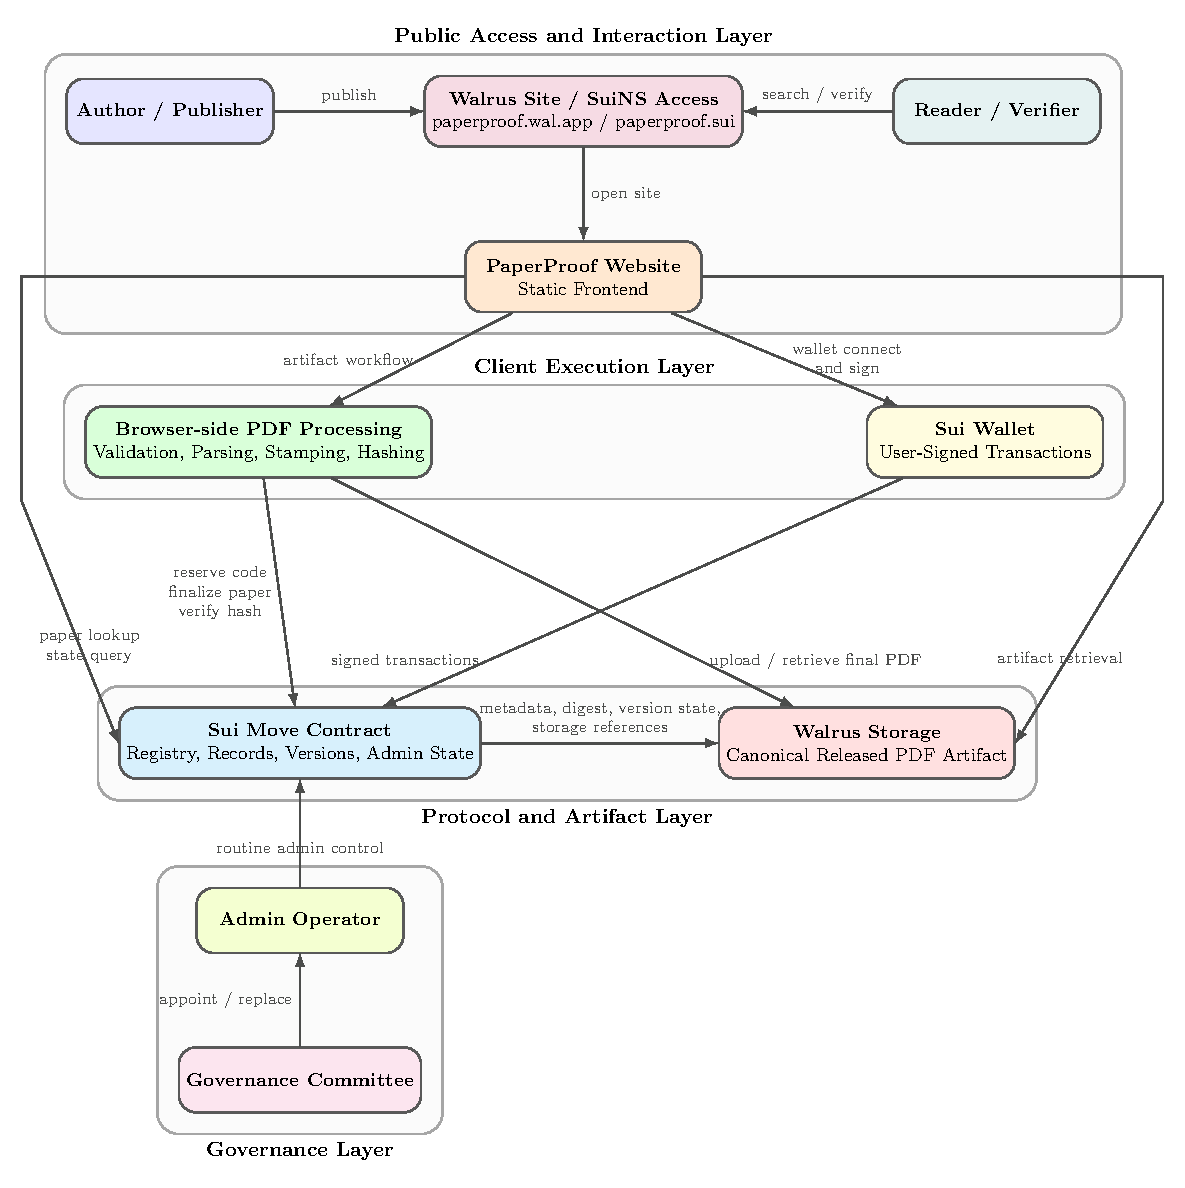
\includegraphics[width=\linewidth]{system-architecture.pdf}
    \caption{System architecture of PaperProof. Authors and readers access the system through the public website and naming layer, while browser-side logic, the Sui contract, Walrus storage, and the lightweight governance layer jointly support decentralized publication and verification.}
    \label{fig:system_architecture}
\end{figure*}

At a high level, the system can be understood as five cooperating layers:

\begin{enumerate}
    \item the frontend interaction layer,
    \item the browser-side document processing layer,
    \item the Sui contract layer,
    \item the Walrus artifact storage layer, and
    \item the governance and administrative control layer.
\end{enumerate}

These layers together support the complete PaperProof lifecycle: metadata entry, paper code reservation, canonical artifact formation, decentralized storage upload, on-chain publication finalization, later retrieval, and independent verification.

\subsection{Frontend Interaction Layer}

The frontend is implemented as a static decentralized web application. Its role is to provide a usable public interface for the PaperProof workflow without acting as the ultimate authority for publication truth.

The frontend is responsible for:
\begin{itemize}
    \item wallet connection,
    \item metadata entry,
    \item local draft management,
    \item PDF selection,
    \item PDF stamping orchestration,
    \item Walrus upload orchestration,
    \item paper search and lookup,
    \item local verification assistance,
    \item presentation of publication and version information.
\end{itemize}

This layer is intentionally lightweight. It does not hold private keys, does not maintain a privileged publication database, and does not determine authoritative publication state independently of the contract. Instead, it serves as an orchestration and usability layer on top of decentralized state and storage.

This architectural choice supports public deployment through a static site model, reduces backend operational burden, and keeps the trust surface comparatively narrow.

\subsection{Browser-Side Document Processing Layer}

A distinctive component of PaperProof is its browser-side document processing logic. This layer operates locally on the user's selected PDF and performs artifact-related operations before publication is finalized.

Its responsibilities include:
\begin{itemize}
    \item validating the selected file as a PDF,
    \item extracting limited preview metadata such as candidate title and abstract,
    \item embedding the reserved paper code into the final PDF,
    \item recomputing file-level properties for the stamped artifact,
    \item computing the SHA-256 hash of the final released PDF,
    \item supporting local verification of downloaded artifacts.
\end{itemize}


This layer is important because PaperProof does not treat the original uploaded file as the canonical published object. Instead, the browser transforms the source document into the final publication artifact by embedding the paper code before the document is uploaded to Walrus and finalized on Sui.

By performing this transformation locally, the system avoids the need for a centralized server to construct or hold the final artifact on behalf of the user. As a result, the browser becomes the site of canonical artifact formation, while the contract and storage layers become the sites of canonical artifact registration and persistence.

\subsection{Sui Contract Layer}

The Sui Move contract is the authoritative state layer of PaperProof. It records publication facts that require strong integrity, explicit state transitions, and public auditability.

The contract is responsible for:
\begin{itemize}
    \item reserving unique paper codes,
    \item recording publication lifecycle state,
    \item storing paper metadata,
    \item maintaining append-only version structure,
    \item binding Walrus storage references,
    \item binding cryptographic file hashes,
    \item managing ownership transitions,
    \item supporting administrative control and governance-related operations.
\end{itemize}


This layer is centered on objects such as the registry, paper record, and version record. These objects together define the identifier space, the publication lifecycle, and the historical structure of a paper.

The contract is also where publication state becomes explicit. A paper can exist in a reserved state before formal release, then transition to a published state when metadata and final artifact facts are committed. This stateful design distinguishes PaperProof from simpler notarization-style approaches that only record a file hash or a storage pointer without a richer publication model.

\subsection{Walrus Artifact Storage Layer}

Walrus serves as the canonical storage layer for the final released PDF artifact. In PaperProof, Walrus is not a decorative storage integration or a secondary archival layer. It is the primary storage substrate for the published document that readers later retrieve and verify.

This layer is responsible for:
\begin{itemize}
    \item storing the final stamped PDF,
    \item exposing blob-related identifiers,
    \item preserving artifact availability through decentralized storage semantics,
    \item supporting later retrieval of the canonical published artifact,
    \item providing storage-related values that can be recorded on-chain.
\end{itemize}


PaperProof relies on Walrus because the system requires more than a generic file upload destination. The final released artifact must remain externally referencable, tied to a storage identity, and usable in later verification. Walrus fits this model by separating artifact persistence from contract state while still allowing the contract to bind the published record to concrete storage-layer references.

This architectural split allows large PDF files to remain off-chain while preserving verifiable linkage between publication facts and publication content.

\subsection{Governance and Administrative Control Layer}

Although PaperProof is primarily a publication system, it also includes a minimal but explicit governance-oriented control layer for administrative continuity.

This layer is responsible for:
\begin{itemize}
    \item defining who acts as the operational administrator,
    \item supporting administrative actions such as pausing and configuration updates,
    \item providing safer operator succession through OpenZeppelin \texttt{two\_step\_transfer},
    \item establishing a path toward stronger governance extensions without requiring a full DAO in the current version.
\end{itemize}


The current architecture separates governance legitimacy from routine execution. A governance committee determines who should serve as the administrative operator, while the operator directly holds the operational authority object and performs day-to-day contract administration. This design preserves practicality while reducing raw single-address administrative fragility.

In addition, this layer provides a foundation for future governance-related extensions, including governance configuration records, committee multisig execution, and treasury control.

\subsection{Trust Boundaries}

A central architectural feature of PaperProof is that different layers carry different trust assumptions.

The frontend is trusted for usability, workflow guidance, and local orchestration, but not as the final authority for publication truth.

The browser-side processing layer is trusted by the author to construct the final artifact locally, but the resulting artifact is later anchored through contract state and Walrus storage rather than through private browser memory.

The Sui contract layer is the authoritative source for publication state, version records, metadata binding, and file hash registration.

The Walrus layer is the authoritative source for the storage identity and retrievable content of the final published PDF.

The governance layer is trusted for operational continuity and authority delegation, but it is intentionally limited in the current design to avoid overloading the publication system with prematurely heavy governance machinery.

This separation of trust is one of the defining architectural properties of PaperProof. The system is not trustless in an absolute sense, but it is structured so that no single website backend must be trusted as the exclusive source of paper existence, artifact identity, and version truth.

\subsection{Deployment-Oriented Architecture}

PaperProof is also designed with deployment realism in mind. The architecture supports a public-facing static site, a live Sui mainnet contract, Walrus-backed PDF artifact storage, and documentation-oriented public access through a lightweight frontend.

This means that the same architecture used during development can also support a live product deployment without introducing a large centralized backend or a separate custodial publication service. The result is a system that is not only conceptually decentralized, but also operationally lightweight enough to remain practical as a public-facing application.

\subsection{Architectural Summary}

The architecture of PaperProof is defined by a clear division of responsibility:
\begin{itemize}
    \item the frontend handles interaction,
    \item the browser constructs the canonical final artifact,
    \item the Sui contract records publication truth,
    \item Walrus stores the released PDF,
    \item the governance layer provides lightweight operational continuity.
\end{itemize}


This layered design allows PaperProof to function as a live decentralized scholarly publication system in which paper registration, artifact release, storage persistence, later verification, and administrative control remain coherent parts of a single end-to-end workflow.

\section{Publication and Verification Workflow}

\subsection{Workflow Overview}

PaperProof is designed as a stateful publication and verification workflow that transforms a local academic PDF into a verifiable decentralized publication artifact. The workflow is not modeled as a single opaque upload event. Instead, it is organized as a sequence of explicit stages, each of which produces a meaningful system state or artifact transition.
\begin{figure*}[!ht]
    \centering
    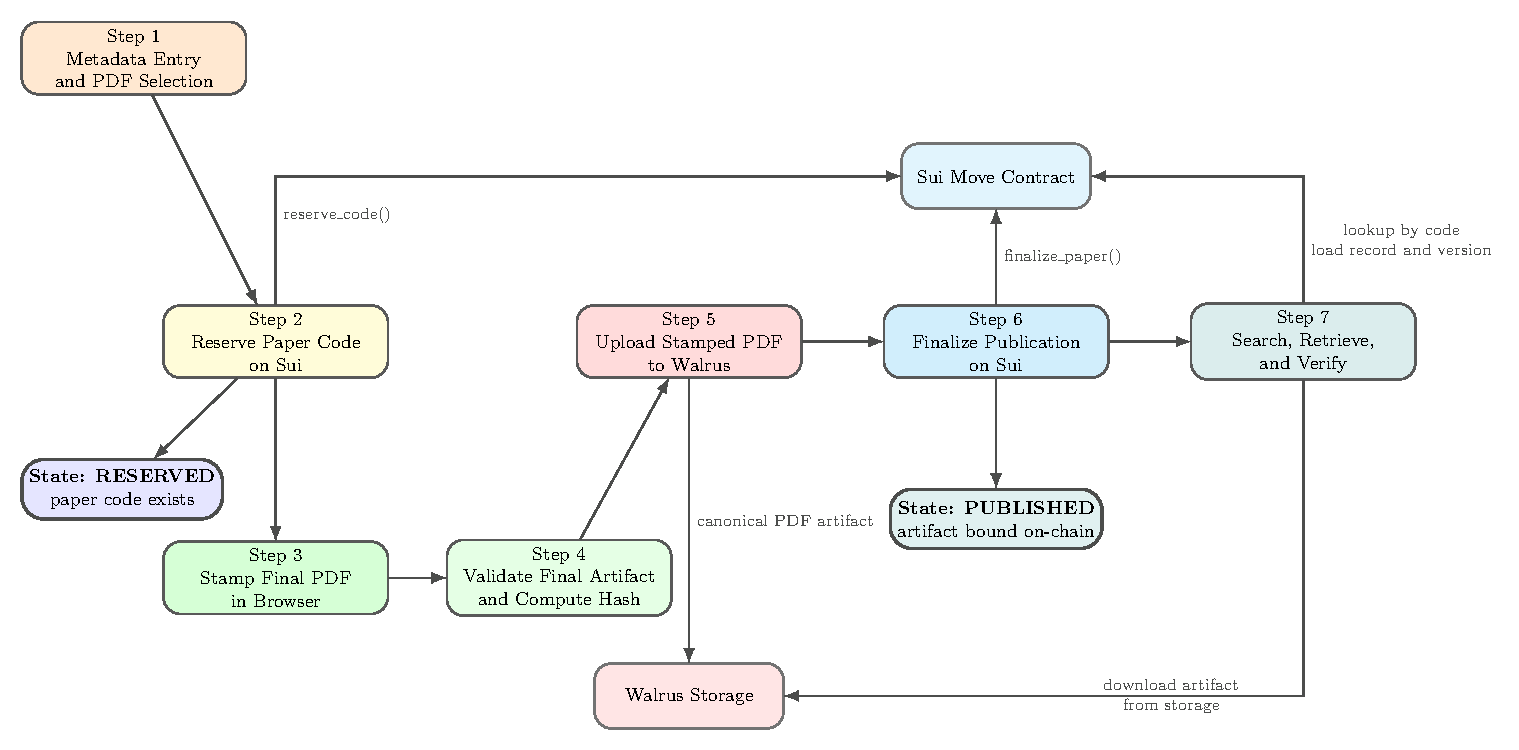
\includegraphics[width=0.95\textwidth]{publication-workflow.pdf}
    \caption{Publication workflow of PaperProof. The workflow proceeds from metadata preparation and code reservation to browser-side artifact formation, Walrus upload, and on-chain publication finalization, with explicit RESERVED and PUBLISHED lifecycle states.}
    \label{fig:publication_workflow}
\end{figure*}

At a high level, the workflow consists of:

\begin{enumerate}
    \item metadata preparation and PDF selection,
    \item paper code reservation,
    \item canonical artifact formation,
    \item decentralized storage upload,
    \item on-chain publication finalization,
    \item public retrieval and verification, and
    \item append-only post-publication version updates.
\end{enumerate}

This structure reflects the core PaperProof idea that a scholarly publication artifact should be created, registered, and later verified through a transparent and auditable process rather than through a single platform-defined release boundary.

\subsection{Metadata Preparation and PDF Selection}

The workflow begins when the author opens the publishing interface and prepares the initial publication inputs. These include the paper metadata and the source PDF file.

The metadata layer includes fields such as:
\begin{itemize}
    \item title,
    \item abstract,
    \item field,
    \item license,
    \item authors,
    \item keywords.
\end{itemize}


At this stage, the selected PDF is still only a local source document. It is not yet the published artifact, and no on-chain publication fact has been created. The frontend performs preliminary checks on both metadata and file-level properties in order to reduce obvious invalid submissions before any wallet interaction is required.

The current frontend can also perform limited preview extraction from the first pages of the selected PDF in order to assist the user with title and abstract entry. However, this preview is treated only as a convenience feature. It does not determine authoritative publication metadata on its own.

\subsection{Paper Code Reservation}

Once the user has provided the required metadata and selected the source PDF, the publication process moves to paper code reservation. This step is performed by a wallet-signed call to the Sui contract.

The reservation transaction creates a unique human-readable paper code and records a new paper object in the \texttt{RESERVED} state. The paper code functions as the public identity of the document throughout its lifecycle. Importantly, this identifier is created before the final publication artifact is constructed.

This reservation-first design has several consequences:
\begin{itemize}
    \item it guarantees that the identifier is unique before release,
    \item it creates a durable on-chain publication placeholder,
    \item it records the initial reserver address,
    \item it provides the code that will later be embedded into the PDF itself.
\end{itemize}


A paper in the reserved state is therefore neither nonexistent nor already published. It is a legitimate intermediate object whose publication has begun but has not yet been completed.

\subsection{Canonical Artifact Formation}

After code reservation, PaperProof constructs the canonical publication artifact locally in the browser. The system embeds the reserved paper code into the PDF, producing a new stamped document intended for publication.

This step is fundamental to the PaperProof model. The canonical artifact is not the author's original source PDF, but the final stamped PDF that visibly carries the publication identifier. This stamped document is the object that will be uploaded, hashed, finalized on-chain, distributed to readers, and later verified.

Following stamping, the frontend performs a second validation pass on the resulting document. This includes recomputing the artifact-level properties of the final file, such as:
\begin{itemize}
    \item file size,
    \item page count,
    \item SHA-256 hash.
\end{itemize}


These values are computed for the final stamped PDF, not for the original local input file. This distinction is crucial, because later verification must be performed against the artifact actually published and retrieved, rather than against a pre-publication local variant.

\subsection{Walrus Upload and Storage Registration}

Once the final stamped PDF has been constructed and validated, it is uploaded to Walrus. This step makes the released artifact persistently retrievable through decentralized storage.

The Walrus interaction is performed as a staged process, which may include:
\begin{itemize}
    \item blob registration,
    \item artifact upload,
    \item storage certification or confirmation.
\end{itemize}


The resulting storage-related information includes references such as:
\begin{itemize}
    \item the Walrus blob identifier,
    \item the blob object identifier,
    \item storage lifecycle information,
    \item other storage-state values required by the contract.
\end{itemize}



These values are preserved as workflow outputs and later bound on-chain during publication finalization.

This stage is important because it establishes that the exact artifact later referenced on-chain already exists as a storage-layer object rather than as a merely hypothetical future upload.
\begin{figure*}[!ht]
    \centering
    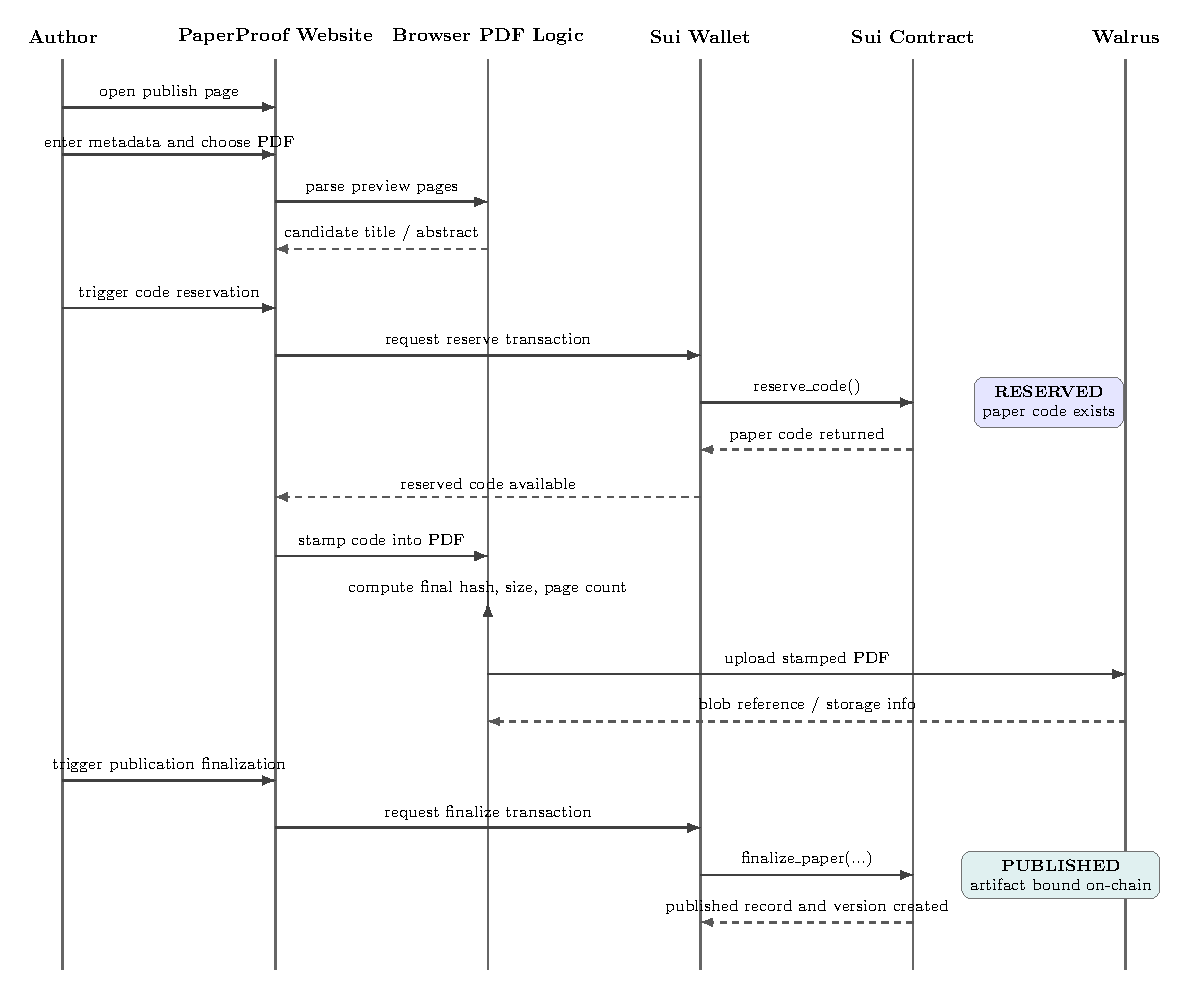
\includegraphics[width=0.95\textwidth]{publish-finalize-sequence.pdf}
    \caption{Publish-and-finalize sequence in PaperProof. The sequence shows how the author, frontend, browser-side PDF logic, wallet, Sui contract, and Walrus interact to reserve a paper code, construct the final stamped artifact, upload it, and finalize publication on-chain.}
    \label{fig:publish_finalize_sequence}
\end{figure*}

\subsection{On-Chain Publication Finalization}

After the final stamped PDF has been uploaded and its file-level facts are known, the user completes publication through an on-chain finalization transaction.

This transaction binds the following to the reserved paper record:
\begin{itemize}
    \item metadata,
    \item Walrus storage references,
    \item file hash,
    \item file size,
    \item page count,
    \item version-related publication information.
\end{itemize}


If the transaction succeeds, the paper moves from \texttt{RESERVED} to \texttt{PUBLISHED}, and the first immutable version record is created.

This is the formal publication event in PaperProof. Before this step, the system only knows that a code has been reserved. After this step, the system contains a complete decentralized publication record linking:
\begin{itemize}
    \item the paper code,
    \item the final released PDF,
    \item the decentralized storage identity of that artifact,
    \item the cryptographic digest used for later verification.
\end{itemize}


\subsection{Public Retrieval and Verification}

Once published, the paper becomes queryable and verifiable through the public PaperProof workflow. A user can retrieve the paper by its code, inspect its current publication state, and access version-related information.

\begin{figure*}[!ht]
    \centering
    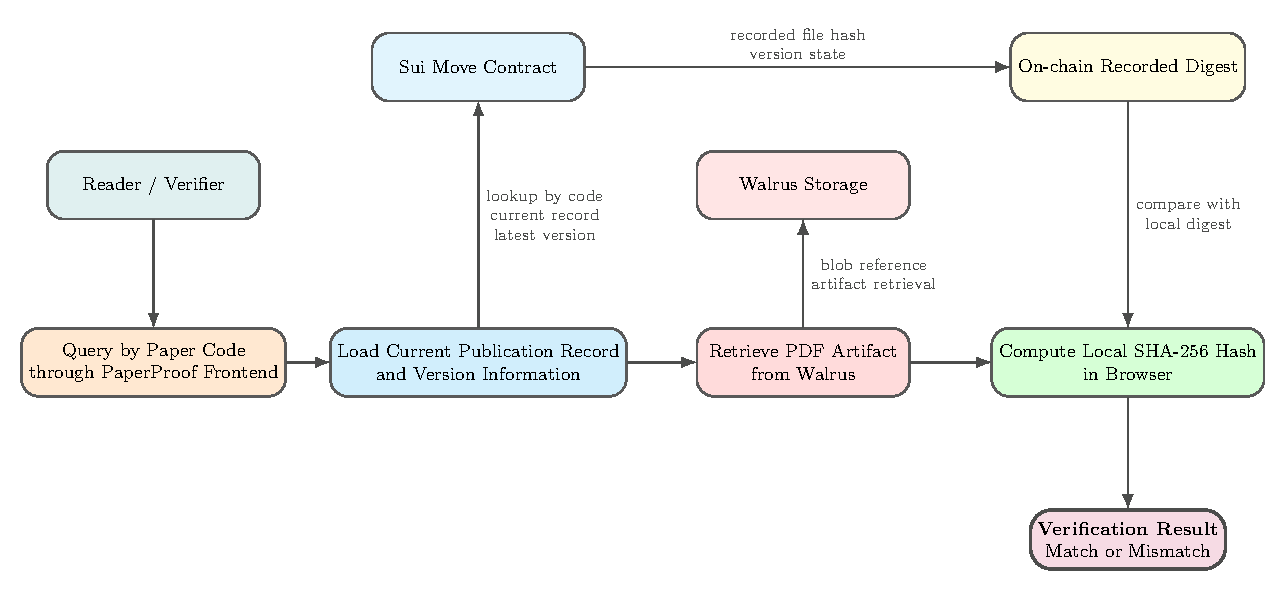
\includegraphics[width=\linewidth]{verification-flow.pdf}
    \caption{Verification flow of PaperProof. A verifier uses the paper code to load publication and version information, retrieves the PDF artifact from Walrus, computes its local hash, and compares it against the on-chain digest.}
    \label{fig:verification_flow}
\end{figure*}

Verification is based on a simple but strong principle: the file retrieved from Walrus should match the cryptographic record stored on-chain.

A later reader or verifier can:

\begin{enumerate}
    \item search the paper by code,
    \item retrieve the current publication record and version information,
    \item download the corresponding PDF artifact from Walrus, and
    \item compute the SHA-256 hash of the downloaded file locally.
\end{enumerate}

If the locally computed digest matches the on-chain digest, the retrieved PDF is verified as the same artifact that was formally published.

\begin{figure*}[!ht]
    \centering
    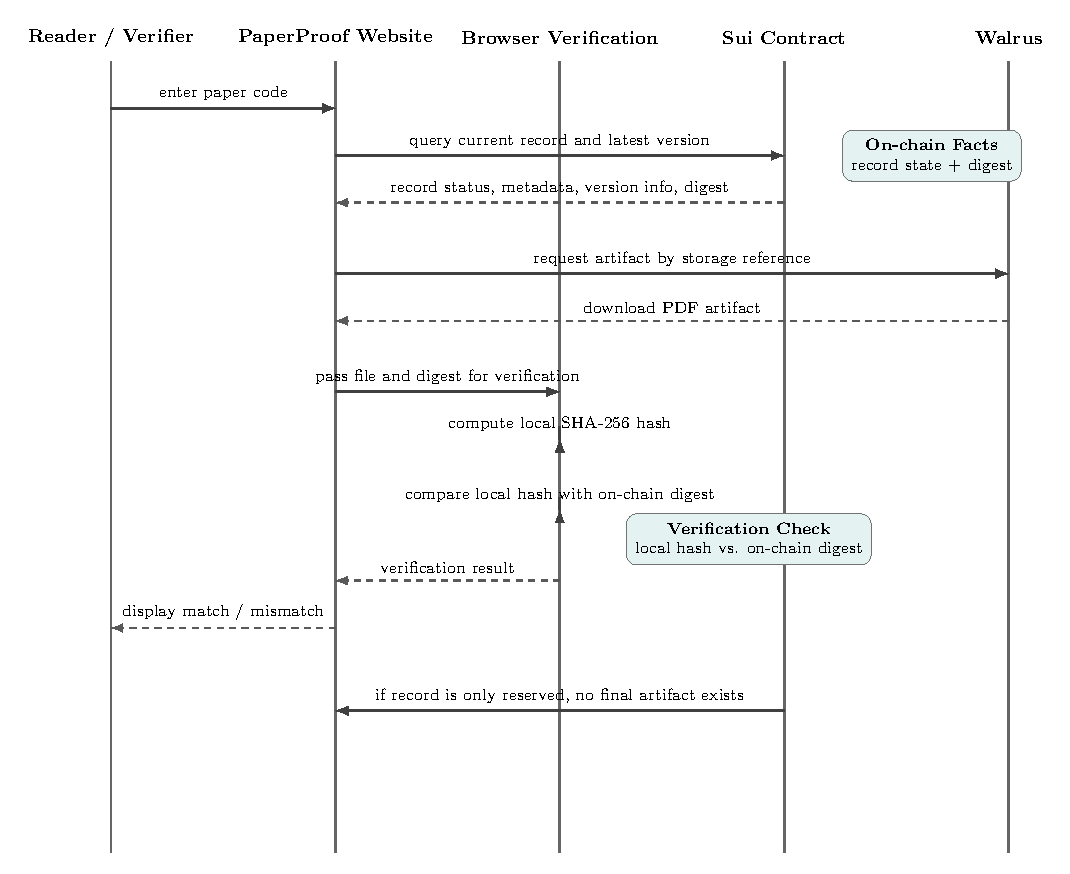
\includegraphics[width=0.95\textwidth]{verification-sequence.pdf}
    \caption{Verification sequence in PaperProof. The reader queries the current publication record on Sui, retrieves the corresponding PDF artifact from Walrus, recomputes the file hash locally, and verifies it against the digest recorded on-chain.}
    \label{fig:verification_sequence}
\end{figure*}

This verification path is central to the PaperProof value proposition. The platform does not ask the user to trust a website statement such as ``this is the correct PDF.'' Instead, it provides enough public information for the user to check the artifact directly.

\subsection{Append-Only Version Update Workflow}

PaperProof also supports post-publication evolution through append-only version updates. When the current paper owner wishes to release a new version, the workflow resembles the initial publication process, but without a new code reservation step.

The update flow is:

\begin{enumerate}
    \item prepare a new local PDF,
    \item stamp it with the existing paper code,
    \item validate the new final artifact,
    \item upload it to Walrus,
    \item finalize it as a new version on Sui.
\end{enumerate}

This creates a new immutable version record rather than overwriting the existing one. Earlier versions remain visible and historically meaningful, while the paper record continues to expose a latest-state view for convenient access.

This append-only structure aligns with the realities of scholarly revision while preserving artifact-level traceability.

\subsection{Recoverability and Failure Tolerance}

Because publication spans browser processing, storage upload, and wallet-signed transactions, interruptions are possible. PaperProof therefore treats several intermediate results as meaningful and reusable.

For example:
\begin{itemize}
    \item a reserved paper code remains valid even if publication is not completed immediately,
    \item a stamped final artifact can be rebuilt or reused,
    \item Walrus upload outputs can be preserved for later retry,
    \item a failed finalization does not invalidate the prior reserved state.
\end{itemize}


This recoverability makes the workflow more resilient than an all-or-nothing publishing interface. It also improves practical usability for a decentralized application, where transactions, wallets, and storage operations may fail independently.

\subsection{Workflow Summary}

The PaperProof workflow is a complete publication-to-verification pipeline built around identifier reservation, canonical final artifact construction, decentralized storage upload, and on-chain publication finalization. The workflow ensures that the released PDF, the storage reference, and the on-chain publication record remain tightly aligned throughout the lifecycle of the paper. In doing so, it transforms decentralized publication from a simple storage exercise into a coherent artifact-based scholarly workflow.

\section{Smart Contract and Data Model}

\subsection{Contract Role in the System}

The Sui Move contract is the authoritative state layer of PaperProof. Its role is to maintain the compact facts that define publication existence, lifecycle state, version identity, ownership, and artifact binding.
\begin{figure*}[!ht]
    \centering
    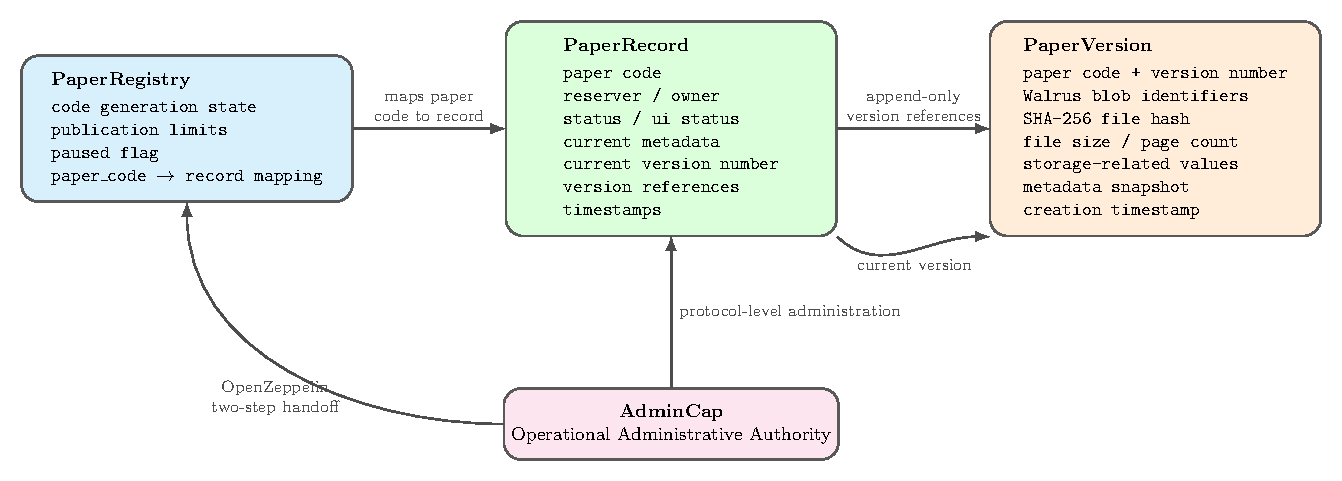
\includegraphics[width=\linewidth]{contract-data-model.pdf}
    \caption{Core contract and data model of PaperProof. The registry anchors identifier generation and lookup, each paper record maintains the current state of a paper, immutable version objects preserve released artifact snapshots, and administrative authority is represented through AdminCap.}
    \label{fig:contract_data_model}
\end{figure*}

The contract does not store the PDF artifact itself. Instead, it records the information necessary to identify, interpret, and verify the artifact, while the file content remains in Walrus. This separation allows the contract to remain focused on publication truth rather than binary storage.

The contract is therefore responsible for:
\begin{itemize}
    \item generating unique paper codes,
    \item recording lifecycle states,
    \item storing current paper metadata,
    \item preserving append-only version records,
    \item binding Walrus storage references,
    \item binding the final PDF hash,
    \item managing ownership transitions,
    \item exposing administrative control points.
\end{itemize}


\subsection{Core Object Model}

The current PaperProof contract revolves around three main publication objects and an administrative authority object.

\subsubsection{PaperRegistry}

\texttt{PaperRegistry} is the global registry object. It acts as the system anchor for code generation, publication lookup, and contract-wide configuration.

Its responsibilities include:
\begin{itemize}
    \item maintaining the identifier-generation state,
    \item storing contract-wide publication limits,
    \item recording whether the system is paused,
    \item mapping paper codes to paper record object identifiers.
\end{itemize}


This object is therefore the entry point for registry-wide publication truth.

\subsubsection{PaperRecord}

\texttt{PaperRecord} is the main state object for a single paper. It represents the current view of the paper and tracks both its publication identity and its latest known state.

A paper record stores information such as:
\begin{itemize}
    \item paper code,
    \item reservation epoch and sequence,
    \item reserver address,
    \item current owner address,
    \item publication status,
    \item UI-related status,
    \item current metadata fields,
    \item current version number,
    \item references to version objects,
    \item timestamps.
\end{itemize}


This object provides the latest-state representation of the paper while also linking to its immutable historical versions.

\subsubsection{PaperVersion}

\texttt{PaperVersion} represents one immutable published version of a paper. Each version captures the file-level and metadata-level facts associated with a particular release.

A version typically stores:
\begin{itemize}
    \item paper code,
    \item version number,
    \item Walrus blob identifier,
    \item Walrus blob object identifier,
    \item SHA-256 file hash,
    \item file size,
    \item page count,
    \item storage-related values,
    \item metadata snapshot,
    \item creation timestamp.
\end{itemize}


This design ensures that every published version remains independently meaningful, even if later versions are added.

\subsubsection{AdminCap}

\texttt{AdminCap} is the operational administrative authority object. It is used for routine contract administration, such as registry pausing, limit updates, and official UI-related administrative actions.

Unlike a raw administrator address field, \texttt{AdminCap} makes authority explicit and object-based. Its custody and succession are handled through OpenZeppelin-based two-step transfer, improving safety and auditability of administrative handoff.

\subsection{Identifier Model}

PaperProof adopts a unique paper code model in which each publication receives a human-readable identifier reserved on-chain before final publication.

The identifier is generated through the registry using epoch-aware state and a monotonic sequence. The result is a code of the form \textit{OriginPaper-\{epoch\}-\{sequence\}} or the equivalent current PaperProof naming format, depending on the deployed version.

The important contract-level properties of the identifier model are:
\begin{itemize}
    \item uniqueness,
    \item non-reusability,
    \item visibility before publication,
    \item direct association with one paper record.
\end{itemize}


This identifier is not merely a UI label. It is a lifecycle anchor that links reservation, stamping, storage, publication, and later verification.

\subsection{Lifecycle State Model}

The paper lifecycle is represented explicitly at the contract level.

\subsubsection{Reserved state}

A paper enters the \texttt{RESERVED} state immediately after code reservation. At this point:
\begin{itemize}
    \item the paper code exists,
    \item the paper record exists,
    \item the reserver is known,
    \item publication has not yet been finalized.
\end{itemize}


This state is meaningful because it represents a legitimate but incomplete publication process.

\subsubsection{Published state}

A paper enters the \texttt{PUBLISHED} state only after finalization has succeeded. At this point:
\begin{itemize}
    \item metadata is bound on-chain,
    \item the final PDF artifact has storage references,
    \item the file hash is recorded,
    \item the first version record exists.
\end{itemize}


This explicit state transition is stronger than treating publication as a loosely defined file-upload event.

\subsection{Metadata Model}

The contract stores both current paper metadata and version-specific metadata snapshots.

Current metadata is held in the paper record for convenience and latest-state access. Immutable historical metadata is preserved in each version object.

The metadata model includes fields such as:
\begin{itemize}
    \item title,
    \item abstract,
    \item authors,
    \item keywords,
    \item field,
    \item license.
\end{itemize}


This dual-layer design prevents later updates from rewriting the historical interpretation of earlier versions while still providing a convenient current-state record.

\subsection{Versioning Model}

Versioning in PaperProof is append-only. A later publication update creates a new \texttt{PaperVersion} object rather than modifying earlier version records.

This has several advantages:
\begin{itemize}
    \item historical versions remain auditable,
    \item file hashes remain tied to the exact artifact of each release,
    \item metadata snapshots remain version-specific,
    \item the paper retains continuity of identity through a stable code.
\end{itemize}

The paper record functions as the mutable latest-state layer, while the version records function as immutable historical artifacts.

\subsection{Ownership Model}

PaperProof distinguishes between several forms of authority.

\subsubsection{Reserver}

The reserver is the address that initially reserves the paper code. In the current model, this address has the authority to complete the first publication finalization of that reserved paper.

\subsubsection{Owner}

The owner is the current paper-level authority after publication. This address can typically add later versions and perform paper ownership transitions where supported.

\subsubsection{Administrator}

The administrator is not a paper-level owner but a protocol-level operator. Administrative authority is represented through \texttt{AdminCap} rather than through ordinary paper ownership fields.

This separation is important because protocol administration and paper authorship are distinct forms of authority.

\subsection{Storage Binding Model}

The contract does not treat storage as a vague external pointer. Instead, it records concrete storage-related values produced by the Walrus publication flow.

These may include:
\begin{itemize}
    \item Walrus blob identifier,
    \item Walrus blob object identifier,
    \item storage end epoch,
    \item shared-blob status.
\end{itemize}


By binding these fields on-chain, the contract makes the relationship between publication fact and storage artifact explicit. This supports later retrieval and verification while keeping file bytes off-chain.

\subsection{Administrative Control Model}

Routine contract-wide management is controlled through \texttt{AdminCap}. The operator holding this object can perform actions such as:
\begin{itemize}
    \item pause or unpause the registry,
    \item update publication-related limits,
    \item update official UI-level moderation or visibility state.
\end{itemize}


Administrative succession uses OpenZeppelin \texttt{two\_step\_transfer}, which provides a safer structured handoff than direct one-step reassignment. This helps reduce accidental operator transfer and makes authority change explicit.

\subsection{Contract Summary}

The PaperProof contract defines a compact but expressive publication state machine. The registry anchors identifier generation and lookup, the paper record provides the latest-state view of each paper, the version objects preserve immutable historical releases, and \texttt{AdminCap} provides structured operational authority. Together, these objects form the core on-chain data model through which scholarly artifacts become reservable, publishable, versionable, and verifiable.



\section{Governance and Administrative Security}

\subsection{Governance Purpose}

PaperProof is primarily a publication and verification protocol, but once deployed as a live public system it also requires an operational governance structure. The system needs a way to maintain administrative continuity, adjust protocol-level configuration, manage official UI-related state, and support safe succession of operational authority.

At the same time, the current project does not require a full on-chain governance engine in order to function. A fully generalized DAO framework would introduce significant complexity, additional attack surface, and a level of institutional machinery that is not yet necessary for the current publication scope. PaperProof therefore adopts a deliberately lightweight governance route.

\subsection{Chosen Governance Route}

The current governance model follows a committee-and-operator structure.

\begin{figure*}[!ht]
    \centering
    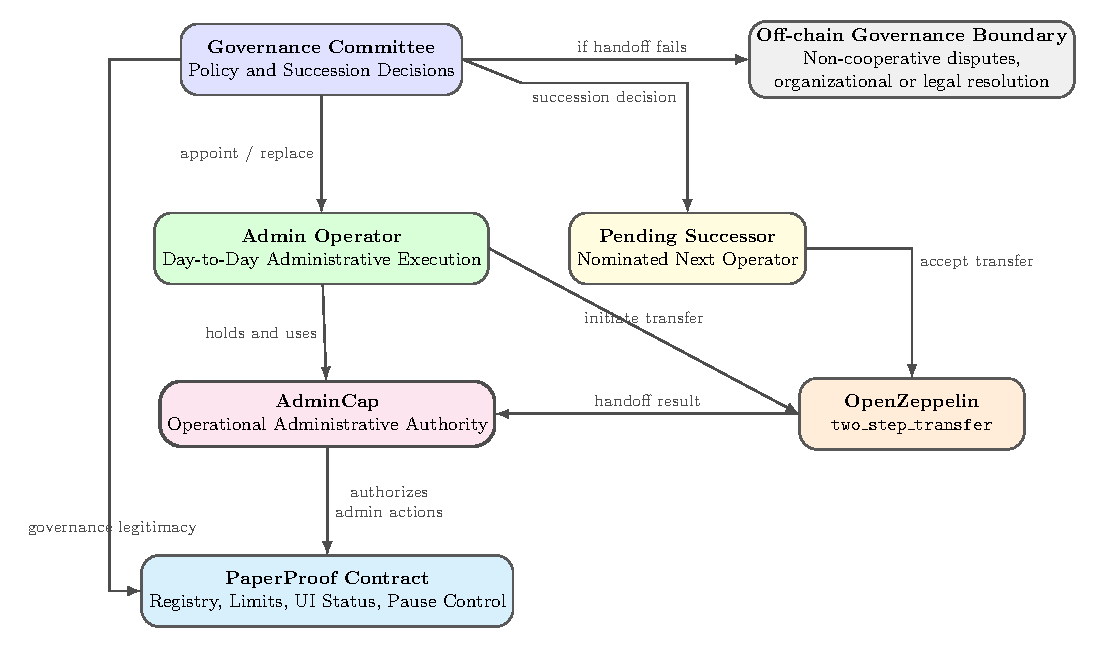
\includegraphics[width=\linewidth]{governance-model.pdf}
    \caption{Governance model of PaperProof. A governance committee determines operator legitimacy, the admin operator directly holds operational authority through AdminCap, and routine protocol administration is separated from higher-level governance legitimacy.}
    \label{fig:governance_model}
\end{figure*}

Under this route:
\begin{itemize}
    \item a governance committee determines who should serve as the operational administrator,
    \item the operational administrator directly holds the protocol administrative authority object,
    \item routine administrative actions are executed by that operator,
    \item administrative succession is protected through OpenZeppelin \texttt{two\_step\_transfer},
    \item committee decisions may be formed off-chain in the current version,
    \item the contract and documentation record governance facts without requiring full on-chain voting.
\end{itemize}


This route is designed to provide a practical balance between safety, clarity, and deployability.

\subsection{Governance Roles}

\subsubsection{Governance Committee}

The governance committee is the highest governance body in the current PaperProof model.

Its responsibilities include:
\begin{itemize}
    \item deciding who should serve as the operational administrator,
    \item deciding when the current operator should be replaced,
    \item defining governance policy,
    \item supervising operator behavior,
    \item guiding future governance evolution.
\end{itemize}


The committee is the source of governance legitimacy, even though its decisions do not yet need to be expressed through an on-chain voting framework for every action.

\subsubsection{Admin Operator}

The admin operator is the day-to-day contract administrator. This role directly holds \texttt{AdminCap} and performs routine protocol-level administrative actions.

Typical operator actions include:
\begin{itemize}
    \item pausing or unpausing the registry,
    \item updating contract-wide publication limits,
    \item applying official UI-level administrative state changes,
    \item participating in operator succession when a handoff is required.
\end{itemize}


The operator is therefore a practical execution role rather than the ultimate source of governance authority.

\subsubsection{Pending Successor}

When the committee decides to change operators, the nominated replacement becomes the pending successor. This role exists during the succession process and becomes the next active operator only after the handoff is completed.

\subsection{Administrative Authority as an Explicit Capability}

A major PaperProof design decision is to represent operational administrative authority through an explicit object, \texttt{AdminCap}, rather than through a raw address stored as a single field.

This improves administrative clarity in several ways:
\begin{itemize}
    \item authority becomes explicit and inspectable,
    \item custody of authority is easier to reason about,
    \item operator succession can be modeled as capability transfer rather than silent address mutation,
    \item administrative security can be improved through structured handoff mechanisms.
\end{itemize}


This design also aligns more naturally with Sui's object-oriented authority model.

\subsection{Why OpenZeppelin Is Used}

PaperProof uses OpenZeppelin specifically for safer administrative handoff. In the current design, OpenZeppelin does not function as a complete governance framework. Instead, its role is narrower and more focused: it strengthens operator succession.

The current system uses OpenZeppelin \texttt{two\_step\_transfer} because administrative authority is too important to move through an unstructured one-step assignment. A safer handoff model reduces the risk of operator replacement errors and makes governance transitions easier to audit.

OpenZeppelin therefore contributes to PaperProof at the capability custody and succession layer rather than at the committee policy layer.

\subsection{Operator Succession Model}

The current PaperProof succession route is based on a two-step handoff.

\begin{figure*}[!ht]
    \centering
    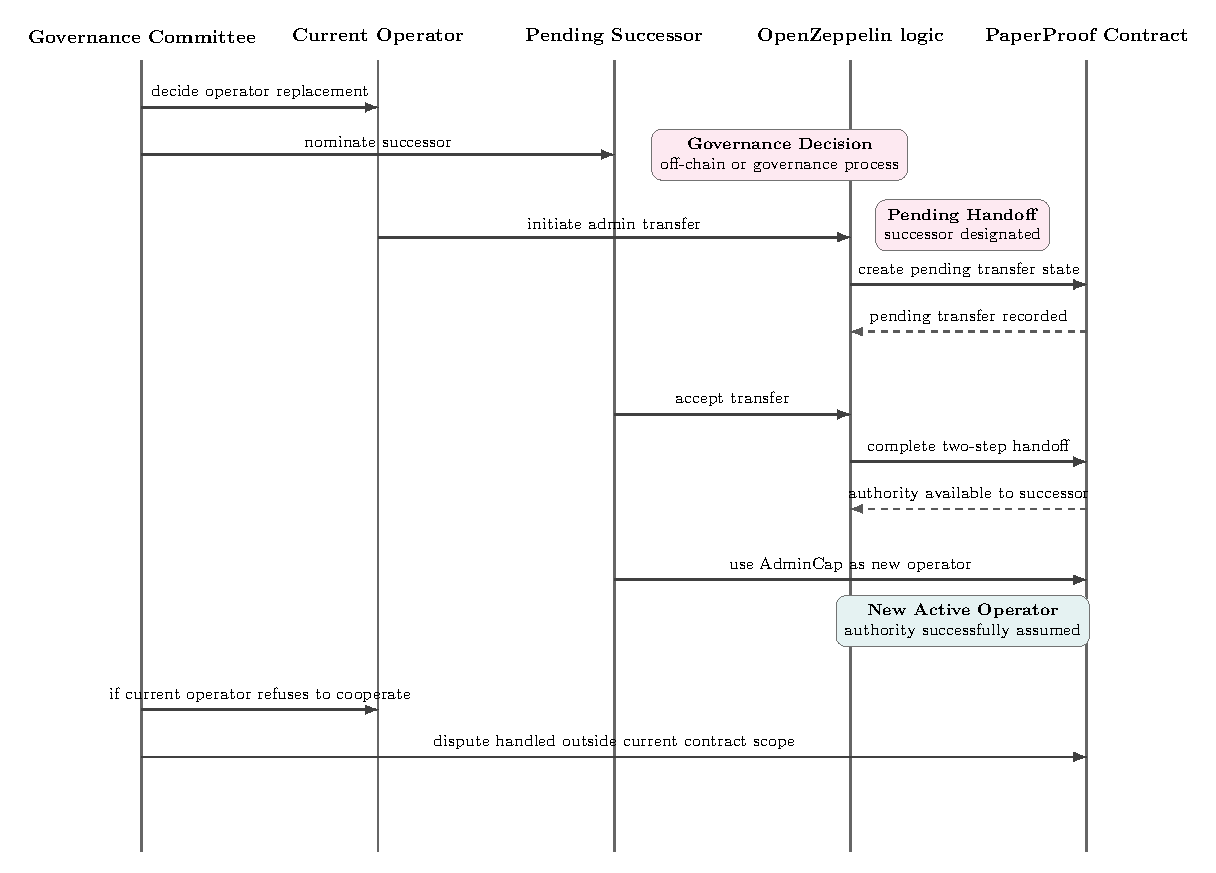
\includegraphics[width=0.95\textwidth]{admin-handoff-sequence.pdf}
    \caption{Administrative handoff sequence in PaperProof. After a governance decision, the current operator initiates authority transfer, the pending successor accepts it through OpenZeppelin two-step transfer, and the new operator becomes the active holder of administrative authority.}
    \label{fig:admin_handoff_sequence}
\end{figure*}

The process is:

\begin{enumerate}
    \item the governance committee decides that a new operator should be appointed,
    \item the current operator initiates transfer of administrative authority,
    \item the nominated successor accepts the transfer,
    \item the successor completes the authority assumption process and becomes the active holder of \texttt{AdminCap}.
\end{enumerate}

This model is safer than direct one-step reassignment because it requires explicit cooperation from the incoming operator and makes the handoff visible as a process rather than as a silent administrative rewrite.

\subsection{Why Full On-Chain Governance Was Deferred}

A stronger governance structure was considered, including possibilities such as:
\begin{itemize}
    \item committee-held administrative capability,
    \item committee-managed multisig execution,
    \item direct on-chain committee member updates,
    \item proposal and approval workflows,
    \item threshold-based governance execution.
\end{itemize}



These designs were judged too heavy for the current PaperProof stage.

The main reasons are:

- publication logic should remain primary,
- governance machinery should not dominate the MVP,
- increased governance complexity would slow implementation and review,
- a working live publication system has higher immediate value than a prematurely maximal governance framework.

The current route therefore prioritizes operational realism over institutional completeness.

\subsection{Governance Configuration Direction}

Although the present governance route is lightweight, it is compatible with a future governance configuration layer that records governance facts more explicitly.

Such a layer may later record:
\begin{itemize}
    \item committee member set,
    \item governance threshold,
    \item governance authority address or multisig identity,
    \item current operator,
    \item pending operator,
    \item governance configuration version.
\end{itemize}


The purpose of such a layer would not necessarily be to encode every committee vote, but rather to expose governance structure and operator legitimacy more transparently.

\subsection{Treasury as a Governance Extension}

A natural future extension of PaperProof governance is the introduction of a protocol treasury. In this model, each formal paper publication may contribute a small amount, such as \texttt{0.01 SUI}, to a treasury controlled under committee-governed authority.

The intended purpose of this treasury is not to transform PaperProof into a financial protocol. Rather, it would serve as:
\begin{itemize}
    \item a lightweight anti-spam friction,
    \item a protocol sustainability reserve,
    \item a governance-controlled operational resource.
\end{itemize}


A treasury extension would make governance materially more meaningful by linking authority not only to administrative settings but also to protocol-level resource stewardship.

Such a treasury can be introduced consistently with the current governance route:
\begin{itemize}
    \item the committee determines treasury policy,
    \item the operator or future treasury operator executes approved actions,
    \item OpenZeppelin-style authority handoff remains relevant for treasury control continuity.
\end{itemize}


\subsection{Treatment of Non-Cooperative Handoffs}

The current governance route deliberately accepts one important boundary: if an outgoing operator refuses to cooperate with a governance-approved succession decision, the current contract does not forcibly seize authority on-chain.

Instead, PaperProof treats that category of dispute as outside the present smart-contract scope and leaves it to:
\begin{itemize}
    \item organizational governance,
    \item social legitimacy,
    \item contractual arrangements,
    \item legal or institutional resolution where applicable.
\end{itemize}


This is an intentional boundary rather than an accidental omission. The current version of PaperProof is designed to make normal authority succession safer and clearer, not to encode every possible adversarial governance conflict.

\subsection{Governance Summary}

PaperProof adopts a lightweight but explicit governance and administrative security model. A governance committee determines operator legitimacy, the operator directly holds \texttt{AdminCap}, and operational succession is secured through OpenZeppelin \texttt{two\_step\_transfer}. This model is intentionally simpler than full on-chain governance, yet significantly stronger than a raw single-address administrator design. It allows PaperProof to remain deployable, understandable, and operationally credible while preserving a clear path toward stronger future governance.

\section{Implementation and Deployment}

\subsection{Implementation Overview}

PaperProof has been implemented as a working decentralized publication system that combines a static web frontend, a Sui Move smart contract, Walrus-backed artifact storage, browser-side PDF processing, and lightweight governance-oriented administrative control. The current implementation is not a conceptual mockup or a purely local prototype. It is intended as a deployable and usable end-to-end workflow for decentralized paper publishing and verification.

The implementation follows the architectural separation described earlier. The frontend provides the public interaction layer, the browser constructs and validates the final publication artifact, the Sui contract records publication facts and version history, Walrus stores the released PDF, and the administrative layer supports protocol-level operational control. These components are integrated into a coherent workflow that can be executed by an end user with a wallet and a local PDF.

\subsection{Frontend Implementation}

The frontend is implemented as a static web application built with a lightweight modern web stack. It is responsible for orchestrating the publication and verification workflow while remaining independent of a privileged application backend.


\begin{figure*}[!ht]
    \centering
    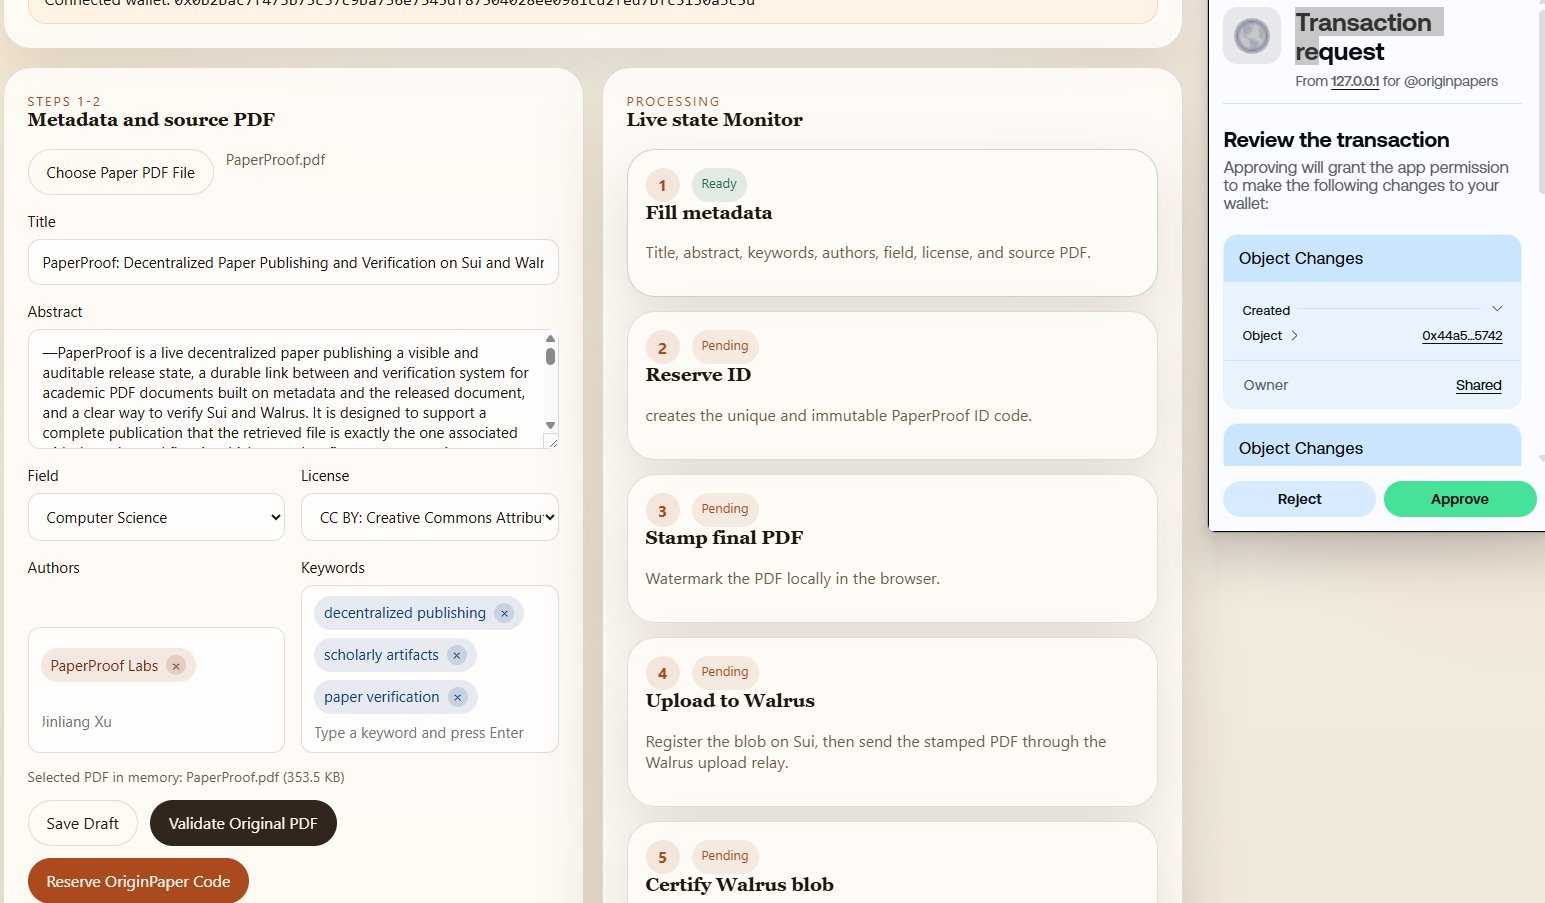
\includegraphics[width=0.96\textwidth]{publishpaper.png}
    \caption{PaperProof publishing interface. The live frontend supports metadata entry, local PDF selection, browser-side artifact preparation, and a staged publication workflow including code reservation, PDF stamping, Walrus upload, and on-chain finalization.}
    \label{fig:publish_interface}
\end{figure*}

Its implemented responsibilities include:
\begin{itemize}
    \item wallet connection and account state display,
    \item metadata collection for publication,
    \item local draft persistence for in-progress publication steps,
    \item PDF selection and validation,
    \item local metadata assistance through limited PDF preview parsing,
    \item browser-side stamping of the final PDF,
    \item Walrus upload orchestration,
    \item publication finalization flow,
    \item paper lookup and detail display,
    \item local artifact verification support,
    \item documentation and governance page rendering.
\end{itemize}


The frontend is intentionally designed to be operationally simple. It does not maintain a server-side publication database, does not custody user private keys, and does not serve as the final authority for publication truth. Instead, it functions as a static orchestration layer over on-chain publication state and decentralized artifact storage.

\subsection{Browser-Side PDF Processing Implementation}

A major implementation feature of PaperProof is that PDF-related processing happens locally in the browser rather than through a centralized file-processing backend.

The current browser-side implementation supports:
\begin{itemize}
    \item file-type checking for uploaded publication files,
    \item limited metadata preview extraction from the first PDF pages,
    \item stamping the reserved paper code into the final PDF,
    \item placing a publication marker in the released artifact,
    \item embedding a PaperProof verification link into the stamped PDF,
    \item recomputing file-level properties for the final artifact,
    \item computing the SHA-256 hash used for later verification.
\end{itemize}


In the current implementation, the browser uses specialized PDF tooling according to task fit. Text extraction for prefill assistance is handled through a PDF parsing library suitable for browser-side page and text analysis, while artifact manipulation and stamping are handled through a PDF generation and modification library better suited to writing and annotating the final document. This separation follows a practical engineering principle: each package is used for the task it performs best, rather than forcing all PDF logic through a single tool.

This browser-side approach is important to the PaperProof trust model. The final canonical artifact is formed on the user side before upload, rather than being reconstructed by a centralized backend.

\subsection{Smart Contract Implementation}

The PaperProof contract is implemented in Sui Move and deployed on Sui mainnet. It acts as the authoritative state machine of the system and records compact publication facts rather than storing PDF bytes directly.

The implemented contract supports the following core functions:
\begin{itemize}
    \item unique paper code reservation,
    \item explicit reserved and published lifecycle states,
    \item publication finalization with metadata and artifact-level binding,
    \item append-only version creation,
    \item paper ownership transfer,
    \item storage-state recording and storage-extension recording,
    \item UI-level moderation state updates,
    \item registry-level configuration updates,
    \item operational administrative control.
\end{itemize}


The contract is structured around the main publication objects described earlier, including the registry object, paper record object, and immutable version objects. Together, these objects realize the identifier model, lifecycle model, metadata model, version model, and verification model of the PaperProof system.

\subsection{Administrative Security Implementation}

The current administrative layer has also been implemented in a more structured form than a raw single-address administrator design. Administrative authority is represented through an explicit \texttt{AdminCap} object rather than solely through an ordinary address field.

Operational administrative handoff uses OpenZeppelin \texttt{two\_step\_transfer}. This means that administrator succession is implemented as an explicit two-step process rather than as an immediate one-step reassignment. The result is a cleaner and safer operational model in which authority transfer is more visible and less error-prone.

Although the current governance route remains lightweight and does not yet implement a full on-chain committee voting framework, the implemented administrative layer already reflects the intended direction of the project: governance legitimacy and operational authority are separated conceptually, and operator succession is treated as a meaningful protocol event rather than as an informal address replacement.

\subsection{Walrus Integration Implementation}

Walrus is integrated as the canonical storage layer for the released PDF artifact. In the implementation, Walrus is not used merely as a generic file bucket. Instead, it is part of the publication workflow itself.

The implemented Walrus-related flow includes:
\begin{itemize}
    \item preparing the final stamped PDF for storage,
    \item registering and uploading the artifact,
    \item recording the resulting blob-related information,
    \item binding Walrus storage references to the paper version on-chain,
    \item later retrieving the artifact for verification.
\end{itemize}


This allows the final released PDF to remain externally retrievable while preserving a direct relationship between storage identity and on-chain publication facts. The contract records the storage-layer references needed to interpret and verify the publication, while Walrus stores the actual binary artifact.

\subsection{Verification Implementation}

PaperProof includes a working verification flow in addition to publication. The implementation allows a user to locate a paper by code, retrieve its publication information, download the corresponding PDF artifact, and compare the downloaded file against the on-chain hash record.

\begin{figure*}[!ht]
    \centering
    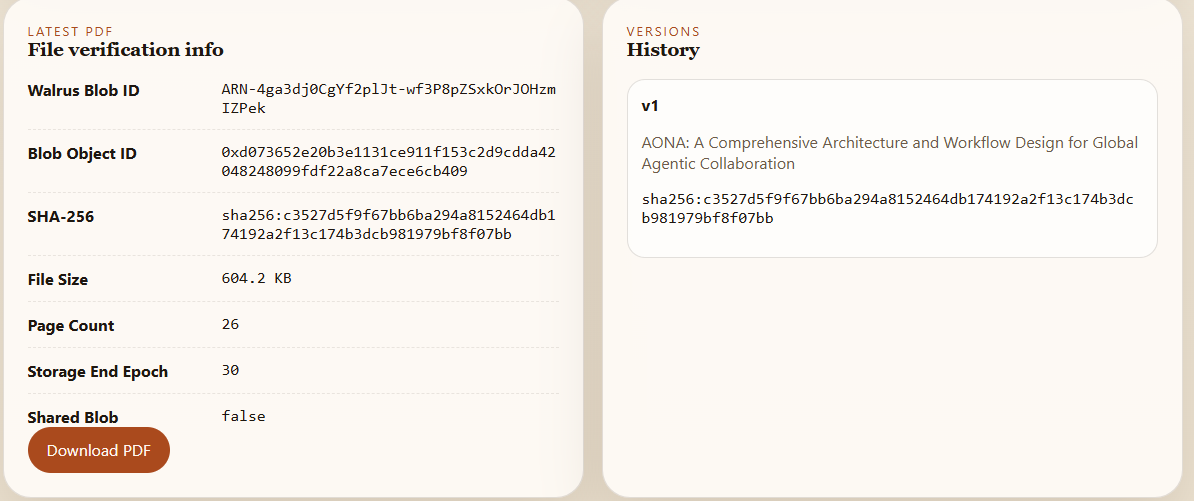
\includegraphics[width=\linewidth]{verification.png}
    \caption{PaperProof verification and artifact information view. The deployed interface exposes artifact-level publication facts, including Walrus identifiers, SHA-256 digest, file size, page count, storage information, and version history for later retrieval and verification.}
    \label{fig:verification_interface}
\end{figure*}

This verification flow is implemented through:
\begin{itemize}
    \item public paper lookup by paper code,
    \item loading the current publication record and version information,
    \item obtaining the Walrus artifact reference,
    \item local hash recomputation in the browser,
    \item comparison against the on-chain digest.
\end{itemize}


This makes verification a concrete user workflow rather than a purely theoretical property of the architecture.

\subsection{Deployment Model}

The PaperProof deployment model reflects the system's emphasis on operational simplicity and decentralized publication truth.

The frontend is deployed as a static site. This means that the public web interface can be served without a custom privileged application backend. The frontend remains replaceable and lightweight, while the authoritative publication facts remain in the Sui contract and the artifact remains in Walrus.

\begin{figure*}[!ht]
    \centering
    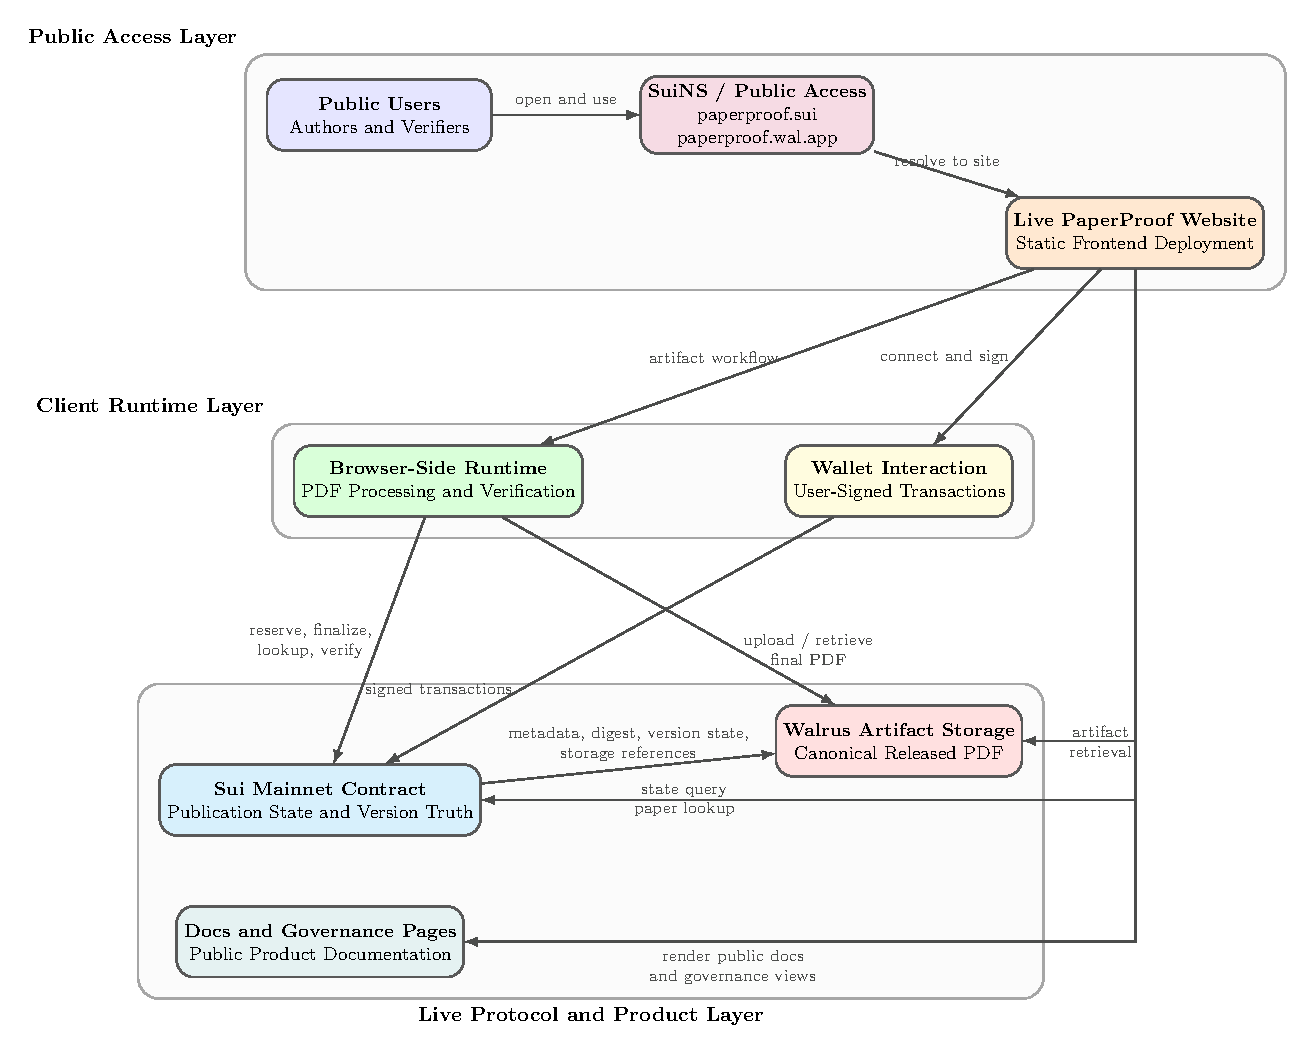
\includegraphics[width=\linewidth]{deployment-product-reality.pdf}
    \caption{Deployment and product reality of PaperProof. The system is publicly accessible through a live website and naming layer, uses browser-side artifact processing and wallet-signed actions, records publication truth on Sui mainnet, and stores the canonical released PDF in Walrus.}
    \label{fig:deployment_product_reality}
\end{figure*}

The contract is deployed on Sui mainnet, which makes the publication workflow a real public on-chain process rather than a local or simulated demonstration. The system therefore supports live wallet interaction, real code reservation, real publication finalization, and public artifact verification.

The storage layer is deployed through Walrus-backed artifact persistence, making the released PDF available through decentralized storage references rather than only through a centralized host.

The public-facing identity layer also benefits from Sui ecosystem naming and access conventions, which help make the deployment more legible and product-like from the user perspective.


\subsection{Public Product Characteristics}

The current PaperProof system exhibits several properties more typical of an early-stage public product than of a purely internal prototype.

First, it provides a complete user-facing workflow rather than a disconnected set of technical demonstrations. A user can open the site, connect a wallet, prepare publication metadata, reserve a paper code, generate the final artifact, upload it, finalize publication, and later verify the released document.

Second, the system has a consistent product identity, including a public-facing name, documentation pages, governance documentation, and a branded publication experience.

Third, the implementation is operationally lightweight. Since the frontend is static and publication truth is externalized to the contract and Walrus, the project does not require a conventional application server for its main publication logic. This significantly reduces hosting and operational complexity relative to traditional web platforms.

These features are important because they show that PaperProof is not only a valid system architecture but also a viable deployment model for a live decentralized publication product.

\subsection{Current Implementation Scope}

The current implementation already supports the central PaperProof workflow, but it remains intentionally scoped.

Implemented capabilities include:
\begin{itemize}
    \item public paper code reservation,
    \item local PDF selection and validation,
    \item browser-side final artifact stamping,
    \item limited metadata prefill assistance,
    \item Walrus upload workflow,
    \item on-chain publication finalization,
    \item public lookup by paper code,
    \item append-only version support,
    \item local file verification by hash,
    \item documentation and governance presentation.
\end{itemize}


Not yet implemented, or deliberately deferred, are broader features such as:
\begin{itemize}
    \item peer review workflows,
    \item scientific quality assessment,
    \item on-chain committee voting,
    \item treasury management,
    \item strong anti-abuse governance,
    \item privacy-oriented document publishing.
\end{itemize}


This implementation scope is consistent with the PaperProof design philosophy: solve decentralized publication and artifact verification first, then consider broader institutional layers later.

\subsection{Deployment Summary}

PaperProof has been implemented and deployed as a live decentralized scholarly publication system. Its current deployment demonstrates that a static frontend, browser-side artifact formation, a Sui Move contract on mainnet, Walrus-based PDF storage, and OpenZeppelin-assisted administrative security can be combined into a functioning publication product. The result is not merely a theoretical architecture, but a usable early-stage protocol and application for decentralized academic artifact publication and verification.

\section{Evaluation and Demonstrated Properties}

\subsection{Evaluation Perspective}

PaperProof is evaluated primarily as a live decentralized publication system rather than as a performance-benchmarking experiment. The current goal of evaluation is therefore not to optimize for throughput, microsecond latency, or adversarial economic simulation. Instead, the evaluation asks whether the implemented system successfully realizes the architectural properties it was designed to achieve.

In particular, the current evaluation focuses on whether PaperProof provides:
\begin{itemize}
    \item identifier-first publication,
    \item canonical binding to the final released artifact,
    \item explicit and visible publication state,
    \item append-only version history,
    \item independent artifact verification,
    \item reduced dependence on a centralized backend,
    \item operationally realistic deployment.
\end{itemize}

This evaluation perspective is appropriate because PaperProof addresses a systems problem of publication integrity and artifact provenance rather than a purely computational optimization problem.

\subsection{Demonstrated End-to-End Workflow}

A first demonstrated property of PaperProof is that the full publication workflow exists as an executable public process rather than as a hypothetical architecture.

The implemented system supports the complete end-to-end sequence:

\begin{enumerate}
    \item a user accesses the public site,
    \item connects a wallet,
    \item enters paper metadata,
    \item selects a local PDF,
    \item reserves a unique on-chain paper code,
    \item stamps the code into the final PDF locally in the browser,
    \item uploads the final artifact to Walrus,
    \item finalizes the paper on Sui,
    \item retrieves the paper later by code,
    \item verifies the downloaded PDF against the on-chain hash.
\end{enumerate}

This end-to-end demonstration is significant because many decentralized publishing concepts stop at isolated features such as file storage, hash anchoring, or metadata registration. PaperProof instead demonstrates a complete publication and verification cycle.

\subsection{Realization of Identifier-First Publication}

A second demonstrated property is the successful realization of identifier-first publication. In PaperProof, a paper code is created before the final released artifact is formed. This is not merely a conceptual design rule; it is directly reflected in the implemented workflow.

The reserved paper code becomes the basis for:
\begin{itemize}
    \item artifact stamping,
    \item later lookup,
    \item version continuity,
    \item verification identity.
\end{itemize}


This confirms that the system does not treat publication identity as a secondary label added after release, but as a foundational part of publication construction itself.

\subsection{Realization of Canonical Final Artifact Binding}

A third demonstrated property is canonical binding to the final released PDF artifact. The system computes file-level properties, including the SHA-256 digest, from the final stamped PDF rather than from the original local source document.

This has a direct verification consequence: the artifact later downloaded from Walrus is intended to be the same object whose hash was recorded on-chain at finalization time. In other words, the contract binds to the actual released publication artifact rather than to an unpublished pre-release file.

This property is central to the PaperProof model and is successfully realized in the current implementation.

\subsection{Realization of Explicit Lifecycle State}

The implemented system also demonstrates a visible and meaningful lifecycle distinction between reserved and published records.

A reserved paper is not treated as nonexistent. Instead, the system explicitly recognizes that publication may begin before artifact finalization is complete. Likewise, publication is not treated as complete until metadata, storage references, and final artifact-level facts have been committed on-chain.

This explicit lifecycle improves the semantic clarity of the system in at least three ways:
\begin{itemize}
    \item it distinguishes valid but incomplete publication from published release,
    \item it allows interrupted workflows to remain meaningful,
    \item it reduces ambiguity about whether a public code corresponds to a finalized paper.
\end{itemize}

\subsection{Realization of Append-Only Version History}

PaperProof also demonstrates append-only versioned publication in practice. Once a paper is published, additional releases can be added under the same paper identity without overwriting historical versions.

Each new release produces a new immutable version object with its own:
\begin{itemize}
    \item artifact reference,
    \item file hash,
    \item metadata snapshot,
    \item storage-related information.
\end{itemize}


Meanwhile, the main paper record continues to present the latest-state view.

This confirms that PaperProof supports document evolution while preserving historical interpretability, which is particularly important in scholarly contexts where revisions may remain relevant for citation, interpretation, and auditability.

\subsection{Realization of Independent Verification}

The system also demonstrates the practical feasibility of artifact verification by later users. A retrieved file can be checked against the on-chain record by recomputing the file hash locally and comparing it with the stored digest.

This is a stronger property than merely making a PDF downloadable. It means that artifact authenticity is not based only on trust in the frontend interface, but can be checked against public decentralized state.

This verification model is one of the clearest ways in which PaperProof differs from conventional document hosting workflows.

\subsection{Realization of Reduced Backend Dependence}

Another demonstrated property is the reduced role of a centralized backend. The current PaperProof workflow does not require a privileged application server to:

\begin{itemize}
    \item assign publication identifiers,
    \item construct the final released PDF,
    \item determine final publication truth,
    \item preserve the authoritative publication record.
\end{itemize}

Instead:
\begin{itemize}
    \item the browser constructs the final artifact,
    \item the contract stores the publication facts,
    \item Walrus stores the released PDF,
    \item the static site orchestrates the workflow.
\end{itemize}


This confirms that the system meaningfully externalizes publication truth beyond a conventional centralized web application architecture.

\subsection{Operational Credibility of the Current Governance Model}

The current lightweight governance route also demonstrates practical credibility for a live early-stage protocol. Although it does not yet implement a full on-chain committee voting system, it already provides a more structured and safer operational model than a raw single-address administrator pattern.

The use of \texttt{AdminCap} and OpenZeppelin \texttt{two\_step\_transfer} demonstrates:
\begin{itemize}
    \item explicit operational authority,
    \item safer administrative handoff,
    \item clearer succession semantics,
    \item a realistic path toward future governance strengthening.
\end{itemize}


This governance layer is therefore not only theoretical documentation; it already affects the implementation of administrative authority and operator succession.

\subsection{Evaluation Summary}

Overall, the current implementation demonstrates that PaperProof successfully realizes the main properties it set out to achieve. It establishes a working identifier-first publication workflow, binds publication truth to the final released artifact, preserves append-only version history, enables later artifact verification, reduces reliance on a trusted backend, and supports operationally meaningful administrative security. These demonstrated properties support the claim that PaperProof is a viable foundation for decentralized scholarly publication and verification rather than merely a conceptual design exercise.


\section{Limitations and Future Directions}

\subsection{Current Scope Limitations}

Although PaperProof provides a working decentralized publication and verification system, its current scope is intentionally limited. The project focuses on publication integrity, artifact provenance, version traceability, and practical deployment rather than on solving every broader problem of scholarly communication.

In particular, the current system does not attempt to provide:
\begin{itemize}
    \item peer review,
    \item scientific quality assessment,
    \item reviewer identity and reputation mechanisms,
    \item recommendation or ranking systems,
    \item citation graph analytics,
    \item plagiarism adjudication,
    \item abuse resolution through fully formalized on-chain governance.
\end{itemize}


This limitation is deliberate. The current PaperProof thesis is that decentralized scholarly infrastructure can already provide meaningful value by improving how papers are identified, published, preserved, and verified, even without solving the entire academic ecosystem in a single system.

\subsection{Governance Limitations}

The current governance route is intentionally lightweight. While this supports practical deployment and clarity, it also leaves several governance capabilities incomplete.

The present version does not yet provide:
\begin{itemize}
    \item full on-chain committee voting,
    \item on-chain proposal and approval workflows,
    \item threshold-based committee execution,
    \item automatic recovery from a non-cooperative operator,
    \item a fully formalized governance configuration object exposed as a complete live protocol layer.
\end{itemize}


As a result, part of governance legitimacy remains external to the contract, particularly in committee deliberation and dispute handling. This is acceptable in the current project stage, but it also defines a clear area for future strengthening.

\subsection{Treasury and Sustainability Limitations}

PaperProof has a credible path toward a governance-controlled treasury, but that extension is not yet fully implemented in the current production workflow. The concept of collecting a small publication contribution, such as \texttt{0.01 SUI}, is attractive for anti-spam friction and protocol sustainability, but it introduces new design questions that remain open.

These include:
\begin{itemize}
    \item how treasury custody should be modeled,
    \item how withdrawal or expenditure authority should be governed,
    \item how protocol maintenance and compensation should be justified,
    \item how treasury policy should remain aligned with PaperProof's scholarly mission.
\end{itemize}


Future treasury work must therefore remain disciplined and governance-aware so that the system does not drift unnecessarily toward financial complexity for its own sake.

\subsection{Artifact and Metadata Limitations}

The current system is centered on PDF publication and verification. This gives the implementation a clear artifact model, but it also narrows the document scope.

At present, the system does not fully address:
\begin{itemize}
    \item richer source-document formats,
    \item structured citation export,
    \item advanced metadata interoperability,
    \item full document semantics beyond PDF-level artifact treatment,
    \item automated extraction of complete scholarly metadata with high reliability.
\end{itemize}

In addition, browser-side metadata assistance currently remains heuristic and limited in scope. It may help prefill title and abstract in some cases, but it is not intended to replace explicit author confirmation of publication metadata.

\subsection{Storage and Persistence Limitations}

Walrus provides an appropriate storage layer for the current PaperProof model, but long-term artifact availability remains a lifecycle issue rather than a one-time solved fact. Storage references, extension needs, shared-blob semantics, and sustainability policies all matter over time.

The current system records storage-related facts and can support storage extension workflows, but broader operational questions remain, such as:

\begin{itemize}
    \item how storage maintenance should be funded long-term,
    \item whether some artifacts should receive subsidy support,
    \item how archival expectations should be communicated to users,
    \item how public interfaces should display storage longevity and maintenance status more clearly.
\end{itemize}

\subsection{User Experience Limitations}

Although PaperProof is a working public product, the current user experience remains early-stage. The system already provides a coherent publication flow, but there is still significant room for improvement in:

\begin{itemize}
\item onboarding clarity,
\item wallet guidance,
\item error handling,
\item publishing feedback,
\item discoverability of published papers,
\item explanation of verification semantics to non-technical users.
\end{itemize}


As a result, the current implementation should be understood as a functioning early-stage product rather than as a highly polished mass-adoption publishing platform.

\subsection{Future Directions}

The future development path of PaperProof can proceed along several complementary directions.

\subsubsection{Stronger governance configuration}

A first direction is to make governance facts more explicit on-chain, including committee composition, thresholds, operator identity, pending successor state, and governance configuration versioning.

\subsubsection{Committee multisig and execution upgrades}

A second direction is to strengthen the relationship between committee legitimacy and on-chain execution, potentially through multisig-backed governance authority and more formal governance update endpoints.

\subsubsection{Treasury implementation}

A third direction is to introduce a governance-controlled treasury that supports anti-spam publication friction, sustainability, and protocol operations without turning PaperProof into an unnecessarily financialized system.

\subsubsection{Richer scholarly metadata support}

A fourth direction is better support for structured authorship, citation-oriented export, more expressive metadata formats, and stronger integration with broader scholarly infrastructure.

\subsubsection{Improved verification and retrieval UX}

A fifth direction is to make verification more legible to ordinary users, with clearer explanations of artifact identity, version meaning, and publication authenticity.

\subsubsection{Broader ecosystem integration}

A sixth direction is deeper integration with other decentralized infrastructure components in the Sui ecosystem, especially where they strengthen scholarly publication, identity, governance, or public artifact discovery.

\subsection{Limitations Summary}

The current limitations of PaperProof do not undermine its central contribution. Rather, they define its scope clearly: PaperProof is an early-stage decentralized scholarly publication protocol focused on artifact publication and verification, not yet a complete academic governance or reputation ecosystem. Its future path lies in strengthening governance, sustainability, metadata richness, and usability while preserving the architectural clarity of its current publication model.

\section{Conclusion}

PaperProof demonstrates that decentralized infrastructure can support a practical and publicly deployable workflow for scholarly PDF publication and verification. By combining identifier-first publication on Sui, browser-side construction of the final stamped artifact, Walrus-backed storage of the canonical released PDF, append-only version history, and OpenZeppelin-assisted administrative handoff, the system establishes a coherent architecture in which publication truth is not reducible to trust in a single web platform.

The current implementation shows that a live decentralized paper publishing product can already provide meaningful value without attempting to solve every surrounding institutional problem of scholarly communication. PaperProof does not seek to replace peer review, editorial judgment, or scientific quality assessment. Instead, it focuses on a narrower but foundational problem: how to reserve a publication identity, release a canonical document artifact, preserve version history, and later verify the retrieved file in a trust-minimized manner.

As an early-stage deployed system, PaperProof also demonstrates that Web3 infrastructure can support non-financial but high-trust public applications in a concrete and usable way. The project already integrates a live website, a Sui mainnet contract, Walrus-based artifact persistence, browser-side PDF processing, and a lightweight governance route with safer administrative handoff. In this sense, PaperProof is not only a technical architecture, but also a functioning protocol prototype and public product for decentralized scholarly artifacts.

More broadly, PaperProof suggests that programmable storage, on-chain state management, and structured authority handoff can be combined to support a new class of verifiable digital publication systems. The value of such systems lies not merely in decentralization as an abstract property, but in making released artifacts more transparent, more durable, and more independently verifiable. PaperProof therefore stands as both a working publication platform and a practical demonstration of how Sui, Walrus, and OpenZeppelin can be used together to build credible public infrastructure for the distribution and verification of digital knowledge artifacts.




%\section*{Acknowledgment}
%This work reflects the current stage of thinking of the corresponding author (xujinliang@caict.ac.cn; jlxufly@gmail.com), and do not necessarily represent the official views of the affiliated institutions.


\bibliographystyle{ieeetr}
\bibliography{Ref}

\end{document}